\chapter{AP-GRAPH: dissection of malware artifacts}
\label{chapter:apgraph}

\begin{quote}
{\itshape
Android markets such as Google Play must continuously protect their users against exposure to malicious applications. In this arms race, up-to-date information is crucial to adapt security solutions to the current malware landscape. However, despite the most recent efforts of the research community, this knowledge is still severely lacking. On the one hand, our understanding of malicious applications comes from private companies who are not willing to share their information. On the other hand, recent techniques developed to characterize malicious applications are generating too much data for manual reviews.

In this chapter, we propose AP-GRAPH as a solution to address these two challenges. AP-GRAPH can analyze large sets of malicious applications at scale and find their most discriminative artifacts based on the partial knowledge provided by antivirus solutions. We evaluated our approach on 1 million Android malware and observed that AP-GRAPH identified the specific characteristics of a dozen of malware families. Moreover, AP-GRAPH is capable of reducing the number of artifacts generated by other characterization approaches to limit the noise generated by such techniques. This information can help the research community in locating the malicious parts hidden inside malware applications and recommend the inspection of suspicious artifacts to security experts.

\vspace{1cm}

\begin{center}
This chapter is based on yet unpublished material.

Database: \url{https://androzoo.uni.lu/apksearch}

Analysis: \url{https://androzoo.uni.lu/apklyze/}
\end{center}
}
\end{quote}

\localtableofcontents{}

To improve the security of Android markets, research groups around the world have developed machine learning based systems that detect malicious applications before they impact mobile users~\cite{burguera_crowdroid:_2011,wang_hey_2012,wu_droidmat:_2012,gascon_structural_2013,zia_droidapiminer:_2013,hutchison_andarwin:_2013,arp_drebin:_2014,chen_finding_2015,alam_droidnative:_2016,mariconti_mamadroid:_2017}.
Even though these systems have been effective in the lab, their adoptions have been comparatively stalled in real-world use cases~\cite{allix_empirical_2016, sommer_outside_2010,canto_large_2017,rossow_prudent_2012}.
One reason to explain this lack of success is that the proposed systems must rely on an extensive set of qualified samples to learn the boundary between benign and malicious applications properly.
Unfortunately, the constant evolution of malicious applications makes the validation of malware samples a bottleneck, as human resources are not sufficient to vet ground truth datasets at such scale~\cite{ics2_cybersecurity_2018}.

As an alternative, the security community relies on antivirus engines to classify malware samples before their use in machine learning experiments.
However, this approach is not without flaws.
Industrial actors do not share the details of their analysis to the public as it would threaten their business model.
At best, antivirus reports provide a condensed label that mentions the type and the name of a malware.
Without a transparent database of knowledge, supervised learning systems cannot be trained for explaining and locating malicious behaviors concealed inside malicious applications.
Moreover, this limitation prevents our community from working with more precise malware definitions and limits our ability to fine-tune our detection systems to the most advanced threats.

In this work, we propose a data mining solution named AP-GRAPH to uncover artifacts associated with malicious behaviors of Android malware families.
With only the information provided by antivirus engines, AP-GRAPH can isolate the specific components of a malware family, categorize their nature and locate their presence inside applications.
The information we collect can then be used for two primary purposes.
On the one hand, security analysts can adopt AP-GRAPH as a triage system to evaluate which artifacts are good candidates and find malicious behaviors in unknown malware samples.
On the other hand, the output of AP-GRAPH can characterize the distinctive aspects of a malware family to complement the use of machine learning based systems and vet large malware ground truth datasets at scale.
\section{Specification of malware artifacts}

\begin{figure*}[!ht]
        \centering
	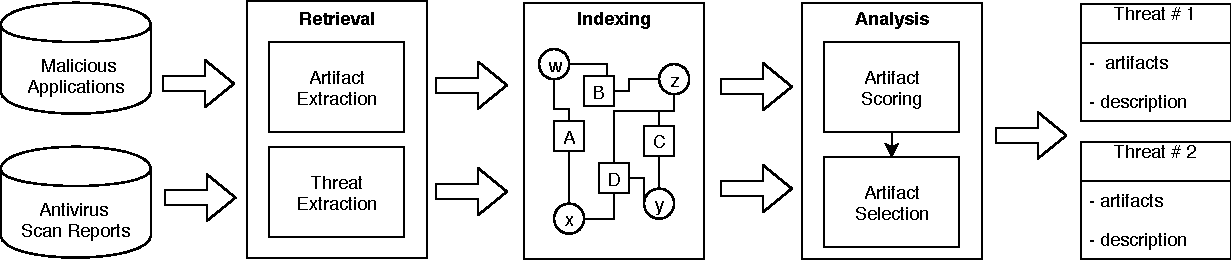
\includegraphics[width=\linewidth]{figures/apgraph/overview.pdf}
        \caption[Architecture of AP-GRAPH]{Architecture of AP-GRAPH divided into 3 stages}
	\label{figure:apgraph:overview}
\end{figure*}

The goal of our approach is to find the internal components that are specific to malware family by using the information publicly available to the security community: a broad set of malicious applications and antivirus scan reports.

The overall approach of AP-GRAPH can be summarized in Figure~\ref{figure:apgraph:overview}.

In this section, we will detail the process used to retrieve, index and analyze this information.
\subsection{Information retrieval}
% \begin{itemize}
%     \item $\mathit{t} \rightarrow$ family
%     \item $\mathit{a} \rightarrow$ artifact
%     \item $\tau \rightarrow$ threshold value
%     \item $\mathit{p} \rightarrow$ application
%     \item $\mathit{g} \rightarrow$ indexing graph
%     \item $\mathit{i} \rightarrow$ artifact identifier
%     \item $\mathcal{M} \rightarrow$ Metric Function
%     \item $\mathcal{S} \rightarrow$ Scanning Function
%     \item $\mathcal{I} \rightarrow$ Indexing Function
%     \item $\mathcal{L} \rightarrow$ Locating Function
%     \item $\mathcal{C} \rightarrow$ Classifier Function
%     \item $\mathcal{E} \rightarrow$ Extraction Function
%     \item $\mathcal{V} \rightarrow$ Verification Function
% \end{itemize}
\subsubsection{Family extraction}
A \textbf{family} $\mathit{t}$ is a name given to a group of malware $\mathit{t} = \{\mathit{p}_1, \mathit{p}_2, ..., \mathit{p}_n\}$ that shares the same artifacts $\{\mathit{a}_1, \mathit{a}_2, ..., \mathit{a}_m\}$.
Given a \textbf{Classifier} $\mathcal{C}$, we define the \textbf{Scanning Function} $\mathcal{S}(\mathit{p}, \mathcal{C}) = \mathit{t}$ that associates a family $\mathit{t}$ to an application $\mathit{p}$.
In this context, an antivirus product can be reduced to a Scanning Function $\mathcal{S}$ that returns a label.
An antivirus label contains various information about the malware, such as its type, name and execution platform.
In our approach, the family is only associated with the name included in the antivirus label.

Unfortunately, extracting information from antivirus labels is not a trivial process, as other researchers found that the naming convention followed by antivirus products is not standard across industrial vendors~\cite{bontchev_current_2005,harley_game_2009}.
Moreover, the ability of antivirus to correctly classify malware varies greatly across products as we demonstrated in Chapter~\ref{chapter:stase}.
In order to collect this information, we rely on EUPHONY Chapter~\ref{chapter:euphony} to achieve state-of-the-art results in unifying the labels of multiple antivirus vendors.

We further note that the selection of families $\{\mathit{t}_1, \mathit{t}_2, ..., \mathit{t}_n\}$ and classifiers $\{\mathcal{C}_1, \mathcal{C}_2, ..., \mathcal{C}_n\}$ is independent of the approach presented in this chapter.
Any clustering of malicious applications can be used as source material in attempting to identify the artifacts specific to a given malware family.
In particular, we note that multiple taxonomies can be tested in parallel, as the extraction of artifacts is independent of the extraction of families during the later stage of the analysis.
The only requirement is that the families provided to AP-GRAPH are associated with more than one malicious applications.
\subsubsection{Artifact extraction}
We define the \textbf{artifact} $\mathit{a}$ of an \textbf{application} $\mathit{p}$ as internal components such that $\mathit{a} \subset \mathit{p}$.
Artifacts are collected through an \textbf{Extraction function} $\mathcal{E}(\mathit{p}) \rightarrow \{\mathit{a}_1, \mathit{a}_2, ..., \mathit{a}_n\}$ associated with either a static or dynamic analysis.
The \textbf{Verification Function} $\mathcal{V}(\mathit{a}, \mathit{p}, \mathcal{E}) \rightarrow \{True, False\}$ can validate that an artifact $\mathit{a}$ either exists or does not exist inside an application $\mathit{p}$, given an Extraction Function $\mathcal{E}$ as a parameter.

The output of the Verification Function $\mathcal{V}$ is represented by a boolean value such that

\begin{itemize}
	\item $\mathcal{V}(\mathit{a}, \mathit{p}, \mathcal{E}) = True$ when $\mathit{a} \subset \mathit{p}$: the artifact $\mathit{a}$ exists inside the application $\mathit{p}$ given the Extraction Function $\mathcal{E}$.
	\item $\mathcal{V}(\mathit{a}, \mathit{p}, \mathcal{E}) = False$ when $\mathit{a} \subset \mathit{p}$: the artifact $\mathit{a}$ does not exist inside the application $\mathit{p}$ given the Extraction Function $\mathcal{E}$.
\end{itemize}

Every artifact $\mathit{a}$ must be encoded by an \textbf{Indexing Function} $\mathcal{I}(\mathit{a}) \rightarrow \mathit{i}$ to guarantee that each $\mathit{a}$ is associated with a unique identifier $\mathit{i}$ and each $\mathit{a}$ can be located unambiguously inside an application $\mathit{p}$.
Thus, the Indexing Function $\mathcal{I}$ is a bijection from the set of artifacts $\{\mathit{a}_1, \mathit{a}_2, ..., \mathit{a}_n\}$ to the set of identifiers $\{\mathit{i}_1, \mathit{i}_2, ..., \mathit{i}_n\}$.
The \textbf{Locating Function} $\mathcal{L}(\mathit{i}) \rightarrow \mathit{a}$ is the inverse of the Indexing Function, such that $\mathcal{L}(\mathcal{I}(\mathit{a})) = \mathit{a}$.

The nature of an artifact $\mathit{a}$ depends on the Extraction Function $\mathcal{E}$ that was chosen for the analysis.
For instance, static analysis retrieves a list of symbols and constants from the source code of an application.
On the other hand, dynamic analysis executes the application to gather system calls and memory footprints.
These elements can constitute a set of artifacts as long as we can define an Indexing Function and a Locating Function for them.
\subsection{Information indexing}
\subsubsection{Data models}

\begin{figure}[!ht]
        \centering
	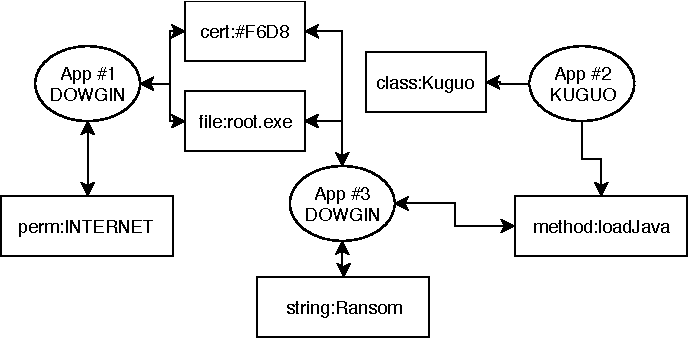
\includegraphics[width=0.8\linewidth]{figures/apgraph/indexes.pdf}
        \caption[Indexing graph produced by AP-GRAPH]{Indexing graph produced by AP-GRAPH: applications are represented as ellipses nodes and artifacts are represented as rectangle nodes.}
	\label{figure:apgraph:graph}
\end{figure}

The \textbf{Indexing Graph} $\mathit{g}$ is a data structure that stores the relations between a set of applications $\{\mathit{p}_1, \mathit{p}_2, ..., \mathit{p}_m\}$ and a set of artifacts $\{\mathit{a}_1, \mathit{a}_2, ..., \mathit{a}_n\}$.
These elements are represented as nodes in the indexing graph and can contain additional attributes such as the family associated with a malicious application.
More formally, the set of nodes of the Indexing Graph can be defined as $\mathcal{N}=\{\mathit{p}_1, \mathit{p}_2, ..., \mathit{p}_m\} \cup \{\mathit{a}_1, \mathit{a}_2, ..., \mathit{a}_n\}$.
The edges of the graph are retrieved by the Verification Function $\mathcal{V}$ and represent the inclusion of an artifact $\mathit{a}$ in an application $\mathit{p}$ when $\mathcal{V}(\mathit{a}, \mathit{p}) = True$.
More formally, the set of edges of the Indexing Graph can be defined as $\mathcal{N}=\{(p_i,a_j) | \mathcal{V}(\mathit{a_j}, \mathit{p_i}) = True \}$.

Figure~\ref{figure:apgraph:graph} shows an example of an Indexing Graph for a small set of applications and artifacts.
Nodes that are applications are represented with elliptical forms and nodes that are artifacts are represented with rectangular forms.
We can see that applications \#1 and \#3 are associated with the \textit{dowgin} family, while application \#2 is associated with the \textit{kuguo} family.
The relation between the applications and the artifacts are represented with arrows in our graph.
Thus, application \#1 is associated with 3 artifacts in this case: perm:internet, cert:\#f6d8 and file:root.exe.
It is also possible that generic artifacts are included by different families, like the artifact method:loadJava which is included by application \#1 (\textit{dowgin}) and \#2 (\textit{kuguo}).
\subsubsection{Data queries}
The main benefit of the Indexing Graph compared to other data structures is that it offers the ability to navigate efficiently between artifacts and applications.
Given an application $\mathit{p}$, we can easily retrieve all the artifacts $\{\mathit{a}_1, \mathit{a}_2, ..., \mathit{a}_n\}$ that are associated with $\mathit{p}$.
Similarly, we can also retrieve all the applications $\{\mathit{p}_1, \mathit{p}_2, ..., \mathit{p}_n\}$ that are associated with artifact $\mathit{a}$.

More formally, let us note  $g$ an Indexing Graph, $p_i$ an application, and $a_j$ an artifact,   we define the following queries that are supported by AP-GRAPH.
For each query, we also provide an example based on the graph from Figure~\ref{figure:apgraph:graph}:

\begin{enumerate}
	% GET /apkfiles/_doc/p
	\item $Q1(\mathit{g}, \mathit{p}) = \{\mathit{a}_1, \mathit{a}_2, ..., \mathit{a}_n\} \in \mathit{p}$: retrieve the set of artifacts $\{\mathit{a}_1, \mathit{a}_2, ..., \mathit{a}_n\}$ that are included in application $\mathit{p}$
	      \begin{itemize}
		      \item {\small $Q1(\mathit{g}, App \#2) = \{class:Kuguo, method:loadJava\}$}
	      \end{itemize}
	      % GET /apkfiles/_search?q=x:a&source=_id
	\item $Q2(\mathit{g}, \mathit{a}) = \{\mathit{p}_1, \mathit{p}_2, ..., \mathit{p}_n\} \ni \mathit{a}$: retrieve the set of applications $\{\mathit{p}_1, \mathit{p}_2, ..., \mathit{p}_n\}$ that include artifact $\mathit{a}$
	      \begin{itemize}
		      \item {\small $Q2(\mathit{g}, method:loadJava) = \{App \#2, App \#3\}$}
	      \end{itemize}
	      % POST /apkfiles/_search?q=x:a&source=labels.family.proposed
	\item $Q3(\mathit{g}, \mathit{a}) = \{\mathit{t} : \mathit{a} \in \mathit{p} \land \mathit{t} \ni \mathit{p} \}$: retrieve the set of families $\{\mathit{t}_1, \mathit{t}_2, ..., \mathit{t}_n\}$ that are associated through the set of applications $\{\mathit{p}_1, \mathit{p}_2, ..., \mathit{p}_n\}$ that includes artifact $\mathit{a}$
	      \begin{itemize}
		      \item {\small $Q3(\mathit{g}, method:loadJava) = \{\textit{dowgin}, \textit{kuguo}\}$}
	      \end{itemize}
	      % POST /apkfiles/_search {"aggs" : { "composite" : { "sources" : [a] } } }
	\item $Q4(\mathit{g}, \mathit{a}) = |\ Q2(\mathit{g}, \mathit{a})\ |$: compute the total number of applications that include artifact $\mathit{a}$
	      \begin{itemize}
		      \item {\small $Q4(\mathit{g}, string:Ransom) = 1$}
	      \end{itemize}
	      % POST /apkfiles/_search {"aggs" : { "composite" : { "sources" : [t, a] } } }
	\item $Q5(\mathit{g}, \mathit{t}, \mathit{a}) = |\ \{\mathit{p} : \mathit{p} \ni \mathit{a} \land \mathit{p} \in \mathit{t} \}\ | $: compute the number of applications associated with family $\mathit{t}$ that include artifact $\mathit{a}$
	      \begin{itemize}
		      \item {\small $Q5(\mathit{g}, DOWGIN, file:root.exe) = 2$}
	      \end{itemize}
\end{enumerate}

\subsection{Information analysis}
\subsubsection{Artifact scoring}
To isolate the artifacts which are specific to families, AP-GRAPH relies on a single metric $\mathcal{M}(\mathit{g}, \mathit{a}) \in [0, 1]$ computed from the queries introduced in the previous section.
This metric quantifies the importance that a single family has compared to the other families.
Thus, if an artifact is present uniformly in multiple families, its $\mathcal{M}$ value will be close to 0.
On the contrary, if the artifact is present mostly in a single family, its $\mathcal{M}$ value will be close to 1.

More formally, we define the metric $\mathcal{M}$ as follow:

$\mathcal{M}(\mathit{g}, \mathit{a}) = \max(\{Q5(\mathit{g}, \mathit{t}, \mathit{a})~ :~ t~ \in~ Q3(\mathit{g}, \mathit{a})\}) / Q4(\mathit{g}, \mathit{a})$

Let us consider a concrete example, where an artifact $\mathit{a}$ appears in 4 families: $\{\mathit{t}_1, \mathit{t}_2, \mathit{t}_3, \mathit{t}_4\}$.
The distribution of artifact $\mathit{a}$ across these families is: $Q5(\mathit{g}, \mathit{t}_1, \mathit{a}) = 100$, $Q5(\mathit{g}, \mathit{t}_2, \mathit{a}) = 200$, $Q5(\mathit{g}, \mathit{t}_3, \mathit{a}) = 200$, $Q5(\mathit{g}, \mathit{t}_4, \mathit{a}) = 1000$ with $Q4(\mathit{g}, \mathit{a}) = 1500$.
The value of the metric, in this case, is $\mathcal{M}(\mathit{g}, \mathit{a}) = \max(100, 200, 200, 1000) / 1500 = 2/3$.
This value is associated with the specificity that the artifact $\mathit{a}$ has on the family $\mathit{t}_4$.
\subsubsection{Artifact selection}

\begin{figure}[!ht]
        \centering
	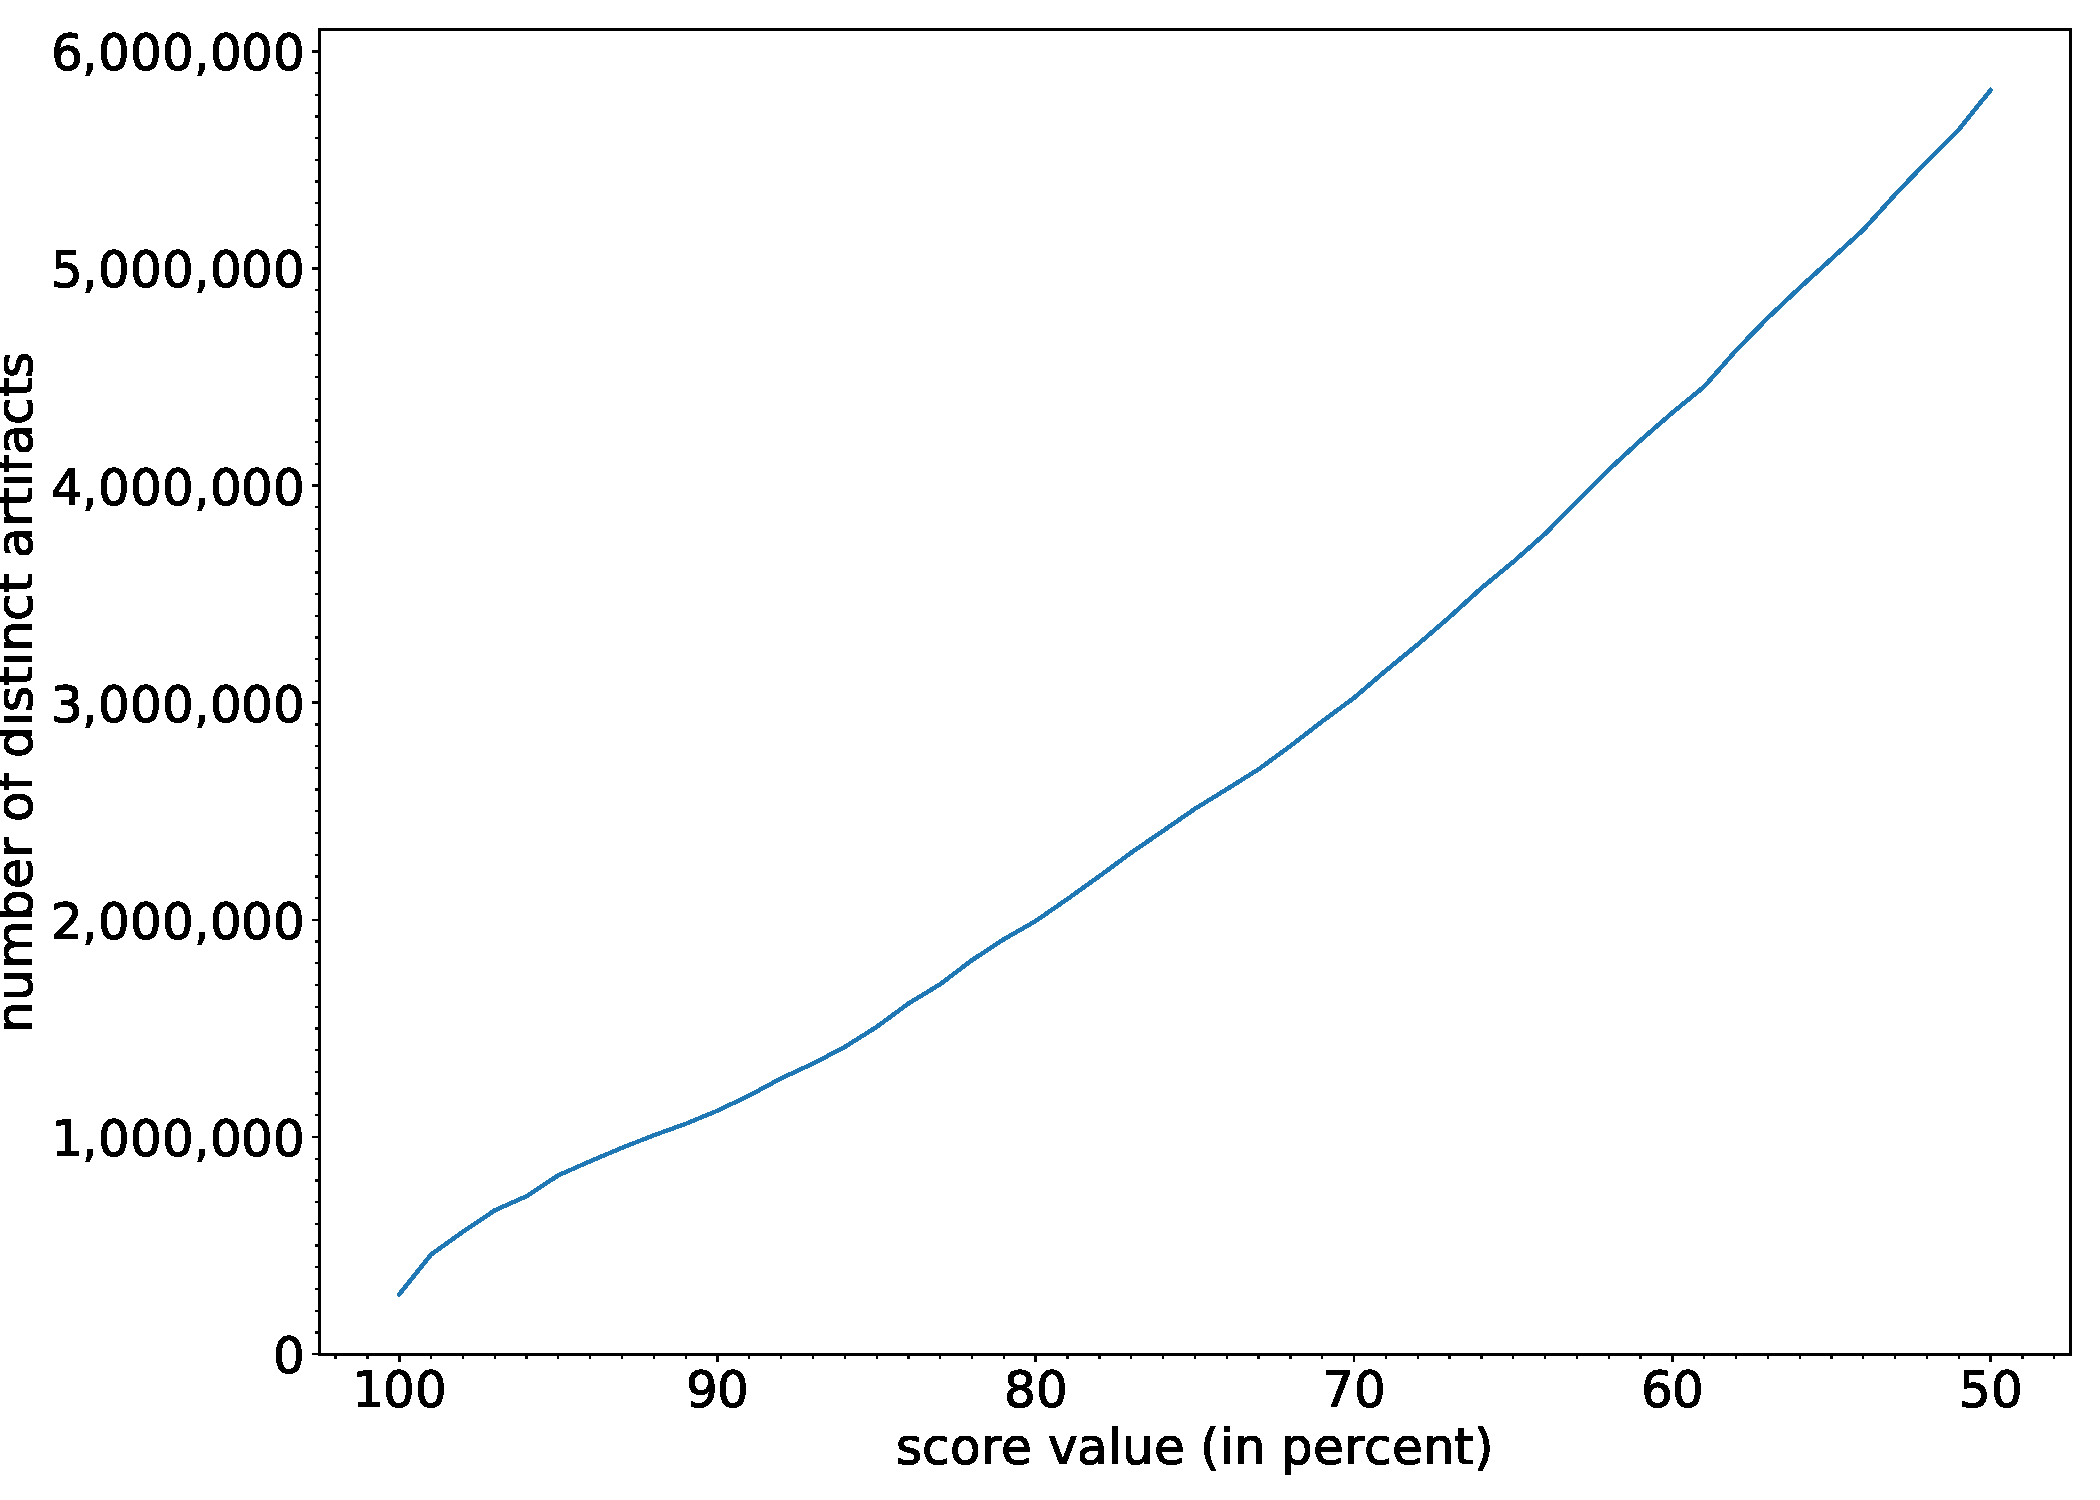
\includegraphics[width=0.8\linewidth]{figures/apgraph/thresholds.pdf}
        \caption[Number of distinct artifacts related to scoring value thresholds]{Number of distinct artifacts related to scoring value thresholds ($\mathcal{M}$)}
	\label{figure:apgraph:thresholds}
\end{figure}

AP-GRAPH use the scoring value $\mathcal{M}$ as a high-pass filter\footnote{a filter that passes values higher than a threshold value} to discriminate the artifacts specific to a single family.
As we described in the previous section, the value of $\mathcal{M}$ will be close to 1 when an artifact appears mostly in a single family.
In particular, the value of $\mathcal{M}$ will be precisely 1 when the artifact is associated with a single family.
While a perfect scoring value would be an excellent theoretical target, antivirus products are known to produce noisy predictions and misclassification as we observed in Chapter~\ref{chapter:stase}.
To take into account this problem, we set a \textbf{threshold value} $\tau$ to reduce our sensitivity to misclassification by antivirus products.

In the absence of ground truth, the threshold value for our analysis is selected based on the information at our disposal.
On Figure~\ref{figure:apgraph:thresholds}, we plot the total number of distinct artifacts retrieved by AP-GRAPH for different values of $\tau$.
We can see that the association between these two variables is linear.
Thus, a smaller value of $\tau$ will uncover more specific artifacts than a higher value.
On the other hand, a smaller value will also include more errors due to antivirus misclassification.

In our analysis, we selected a conservative threshold value of 0.95 to take into account a small amount of noise introduced by antivirus misclassification.
Therefore, the most important family for a given artifact must account for at least 95\% of the total of times an artifact is encountered in malware samples or $\mathcal{M}(\mathit{g}, \mathit{a}) > 0.95$.
For instance, if an artifact appears 1000 times in total, this artifact is considered specific to a family by AP-GRAPH if an only if it is present at least 950 times in this single family.
\section{Creation of malware knowledge base}
In this section, we discuss three architectures designed to support the indexing of malware artifact at scale.

Each part of this section will discuss the trade-off associated with the proposed architectures and their benefits on computing statistics from malware datasets.
\subsection{Architecture A: Datomic}

\begin{figure}[!ht]
        \centering
	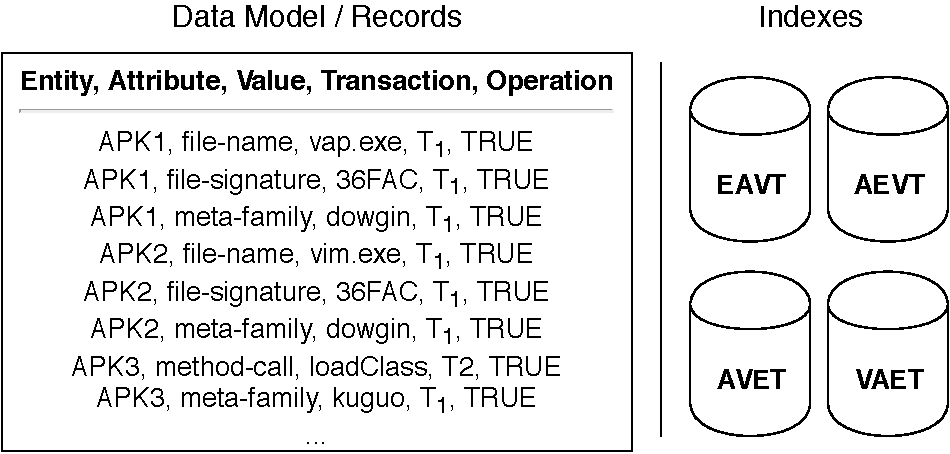
\includegraphics[width=0.75\linewidth]{figures/apgraph/architectures/datomic.pdf}
	\caption{Structure of a knowledge base powered by Datomic}
	\label{figure:apgraph:architectures:datomic}
\end{figure}

Datomic~\cite{cognitech_datomic_nodate} is a commercial database released in 2012 by Cognitech.
The data model of Datomic is inspired by the Resource Description Framework (RDF), as documents are serialized in a 5-tuples containing the entity, attribute, value, transaction, and operation status.
Figure~\ref{figure:apgraph:architectures:datomic} shows an example of tuples associated with three Android malware.
In this example, malware entities are described based on information gathered from static analysis, such as the list of file names and signatures embedded in the application or the list of methods that will be called during its execution.
Datomic features a flexible querying system as records can be saved in four different indexes to support row-oriented (EAVT), column-oriented (AEVT and AVET) and graph-oriented (VAET) access.
Compared to relational database systems, Datomic information are never updated nor deleted and can only be accumulated over time.
Thus, an operator can query the state of the knowledge base at a particular point in time and find the delta that was added before or after a point in time.

Datomic fits the requirements of AP-GRAPH for several reasons.
On the one hand, Datomic supports a wide variety of indexing patterns to optimize the performance of read queries.
The EAVT index can be leveraged to request information about a particular Android application while the AEVT and AVET indexes can be used to compute statistics on the distribution of malware artifacts.
On the other hand, the data schema can be extended with new records, as the Datomic model can be adapted to represent information without impacting the existing structure of the database.

However, Datomic is not suited for use cases that require intensive write operations.
Indeed, Datomic supports ACID properties by limiting the writing process to a single transactor (i.e., a single machine core across the cluster).
Thus, and despite great read performance, Datomic cannot power the indexing of malware ground truth as large as Androzoo~\cite{allix_androzoo:_2016}.
\subsection{Architecture B: Flat file}

\begin{figure}[!ht]
        \centering
	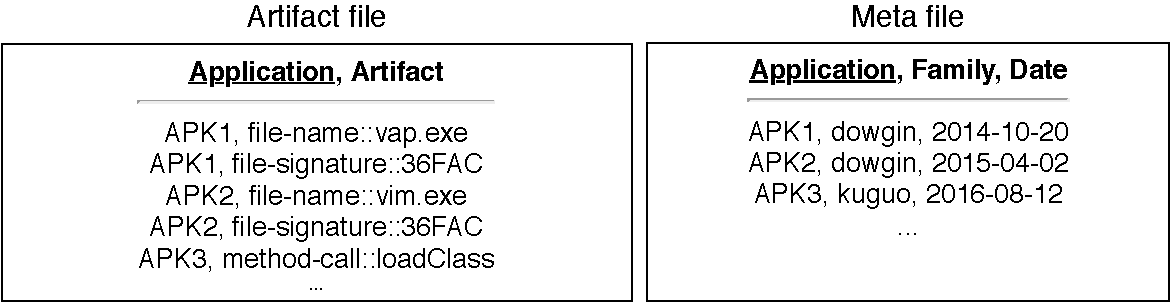
\includegraphics[width=\linewidth]{figures/apgraph/architectures/flat.pdf}
	\caption{Structure of a knowledge base powered by flat files}
	\label{figure:apgraph:architectures:flat}
\end{figure}

Flat files provide a simple format and rely on the operating system to perform read and write operations.
Information can be organized into a delimited file where each line corresponds to a new record.
Figure~\ref{figure:apgraph:architectures:flat} represents two flat files that describes the relationship between applications, artifacts, family and time.
On the one hand, the artifact file, once sorted, can be used to retrieve information by application or by artifact to support the query required by AP-GRAPH.
On the other hand, the meta file can be joined to the artifact file to add additional information that allows the analysis of malware families over time.

However, the simplicity of flat files is both their greatest strength and their greatest weakness.
Flat files do not support indexing or query capabilities found in other database systems beside sequential read and write operations.
Moreover, indexing the artifact file either by application or by artifact requires twice the amount of disk space both for sorting and storing the result file.
In the end, a flat file architecture is a fast prototype solution that works as long as a single machine has enough disk capacity during the sorting process.
\subsection{Architecture C: Elastic}

\begin{figure}[!ht]
        \centering
	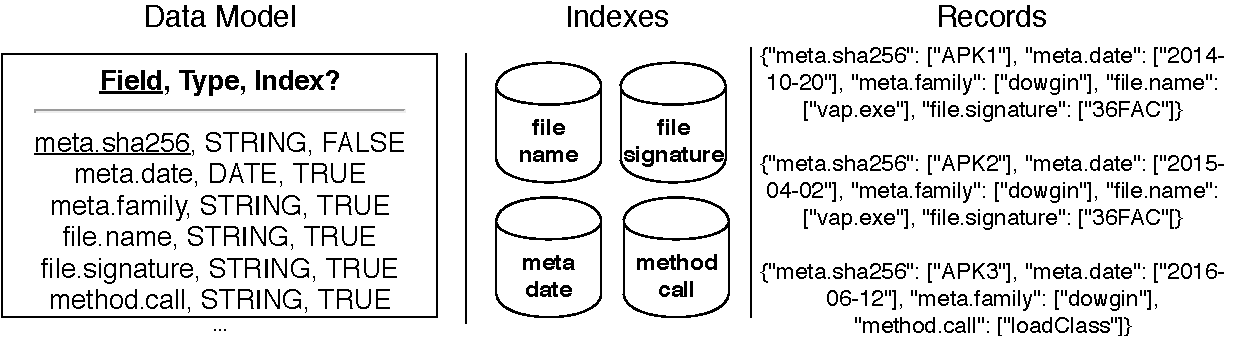
\includegraphics[width=\linewidth]{figures/apgraph/architectures/elastic.pdf}
	\caption{Structure of a knowledge base powered by ElasticSearch}
	\label{figure:apgraph:architectures:elastic}
\end{figure}

Elastic~\cite{elastic_elastic_nodate} is an open source database built to retrieve information from structured documents such as JSON files.
The database has been used by many professional actors to search a large corpus of text, as the indexing capabilities of Elastic are tailored toward this use case.
Moreover, an Elastic cluster can be deployed across multiple computers to aggregate the processing and storing capacity from more than one machine.

Figure~\ref{figure:apgraph:architectures:elastic} presents a structure for an Elastic knowledge base.
Artifacts are listed in a schema file that contains the name, the type and the operation index for the fields.
In Elastic, fields are automatically indexed to enumerate documents that contain them efficiently.
For instance, the file signature '36FAC' is found both in 'APK1' and 'APK2', which means that these two documents will be returned when a user issues a query.

The main benefit of an Elastic based architecture is to power the queries of AP-GRAPH at scale.
The system can retrieve information about a single application, a single artifact or complex analytic queries.
Since data are distributed across multiple machines, computer resources can be shared to speed up the analysis or support more massive ground truth datasets.

However, the solution is the most complex of the three as computer clusters are harder to maintain than a system deployed on a single computer.
Furthermore, while existing documents can be updated to add more fields, this task is a costly operation as it requires to reindex the whole database file.
Hence, this architecture solution should be reserved for complex use cases or when information cannot be stored on a single computer.
\section{Characterization of malware families}
In this section, we report the results of AP-GRAPH in characterizing malware families.

In the first part, we describe the datasets, artifacts, and families comprised in our analysis.
Then, we evaluate the performance of AP-GRAPH in collecting specific artifacts while simultaneously dropping the ones which are not relevant in discriminating malware families.
Finally, we perform a case study analysis to assess the quality of the information retrieved by AP-GRAPH.
\subsection{Dataset}

\begin{table}[t]
	\centering
        \caption[Distribution of applications and malware per market]{Distribution of applications and malware per market (note: an application can be distributed on multiple markets)}
	\begin{tabular}{|c|r|r|r|}
		\hline
                \textbf{Markets}         & \textbf{Malware} & \textbf{Total}     & \textbf{\%}  \\
		\hline
		play.google.com & 579,840 & 4,315,707 & 13  \\
		anzhi           & 501,748 & 742,788   & 67  \\
		appchina        & 334,544 & 593,110   & 56  \\
		mi.com          & 71,584  & 113,583   & 63  \\
		1mobile         & 15,922  & 57,530    & 27  \\
		angeeks         & 17,528  & 55,794    & 31  \\
		slideme         & 8,645   & 52,467    & 16  \\
		praguard        & 0       & 10,186    & 0   \\
		torrents        & 126     & 5,294     & 2   \\
		freewarelovers  & 169     & 4,145     & 4   \\
		proandroid      & 346     & 3,683     & 9   \\
		hiapk           & 1,153   & 2,512     & 45  \\
		fdroid          & 40      & 2,023     & 1   \\
		genome          & 1,247   & 1,247     & 100 \\
		apk\_bang       & 121     & 363       & 33  \\
		unknown         & 0       & 57        & 0   \\
		\hline
	\end{tabular}
	\label{table:apgraph:markets}
\end{table}



The evaluation of AP-GRAPH is based on a large set of Android malware collected by the Androzoo project~\cite{allix_androzoo:_2016}.
This project aims to provide a representative sample of Android applications that other researchers can use in their experiments.
Androzoo contains more than 6 million Android applications gathered from various Android markets.
The dataset also includes nearly 1 million apps considered malicious by at least one antivirus referenced on VirusTotal~\cite{noauthor_virustotal_nodate}.
The distribution of applications and malware per market can be found in Table~\ref{table:apgraph:markets}.
In the Android ecosystem, \textit{play.google.com} is recognized as the official market, while other market places are alternative sources of applications.
From this table, we can observe that alternative markets have a higher proportion of malicious applications than the official market.
\subsubsection{Families}
The families of our evaluation are assembled from Androzoo++~\cite{li_androzoo++:_2017}, a collection of metadata related to the Androzoo dataset.
In particular, this project includes the label of every antivirus referenced on VirusTotal~\cite{noauthor_virustotal_nodate}.
As we noted in Chapter~\ref{chapter:stase}, antivirus labels can provide noisy output and contain various information which are not directly related to the family name.
To handle this lack of consistency, we use EUPHONY to extract the name from antivirus labels and to unify them across multiple antivirus products.

\begin{figure}[!ht]
        \centering
	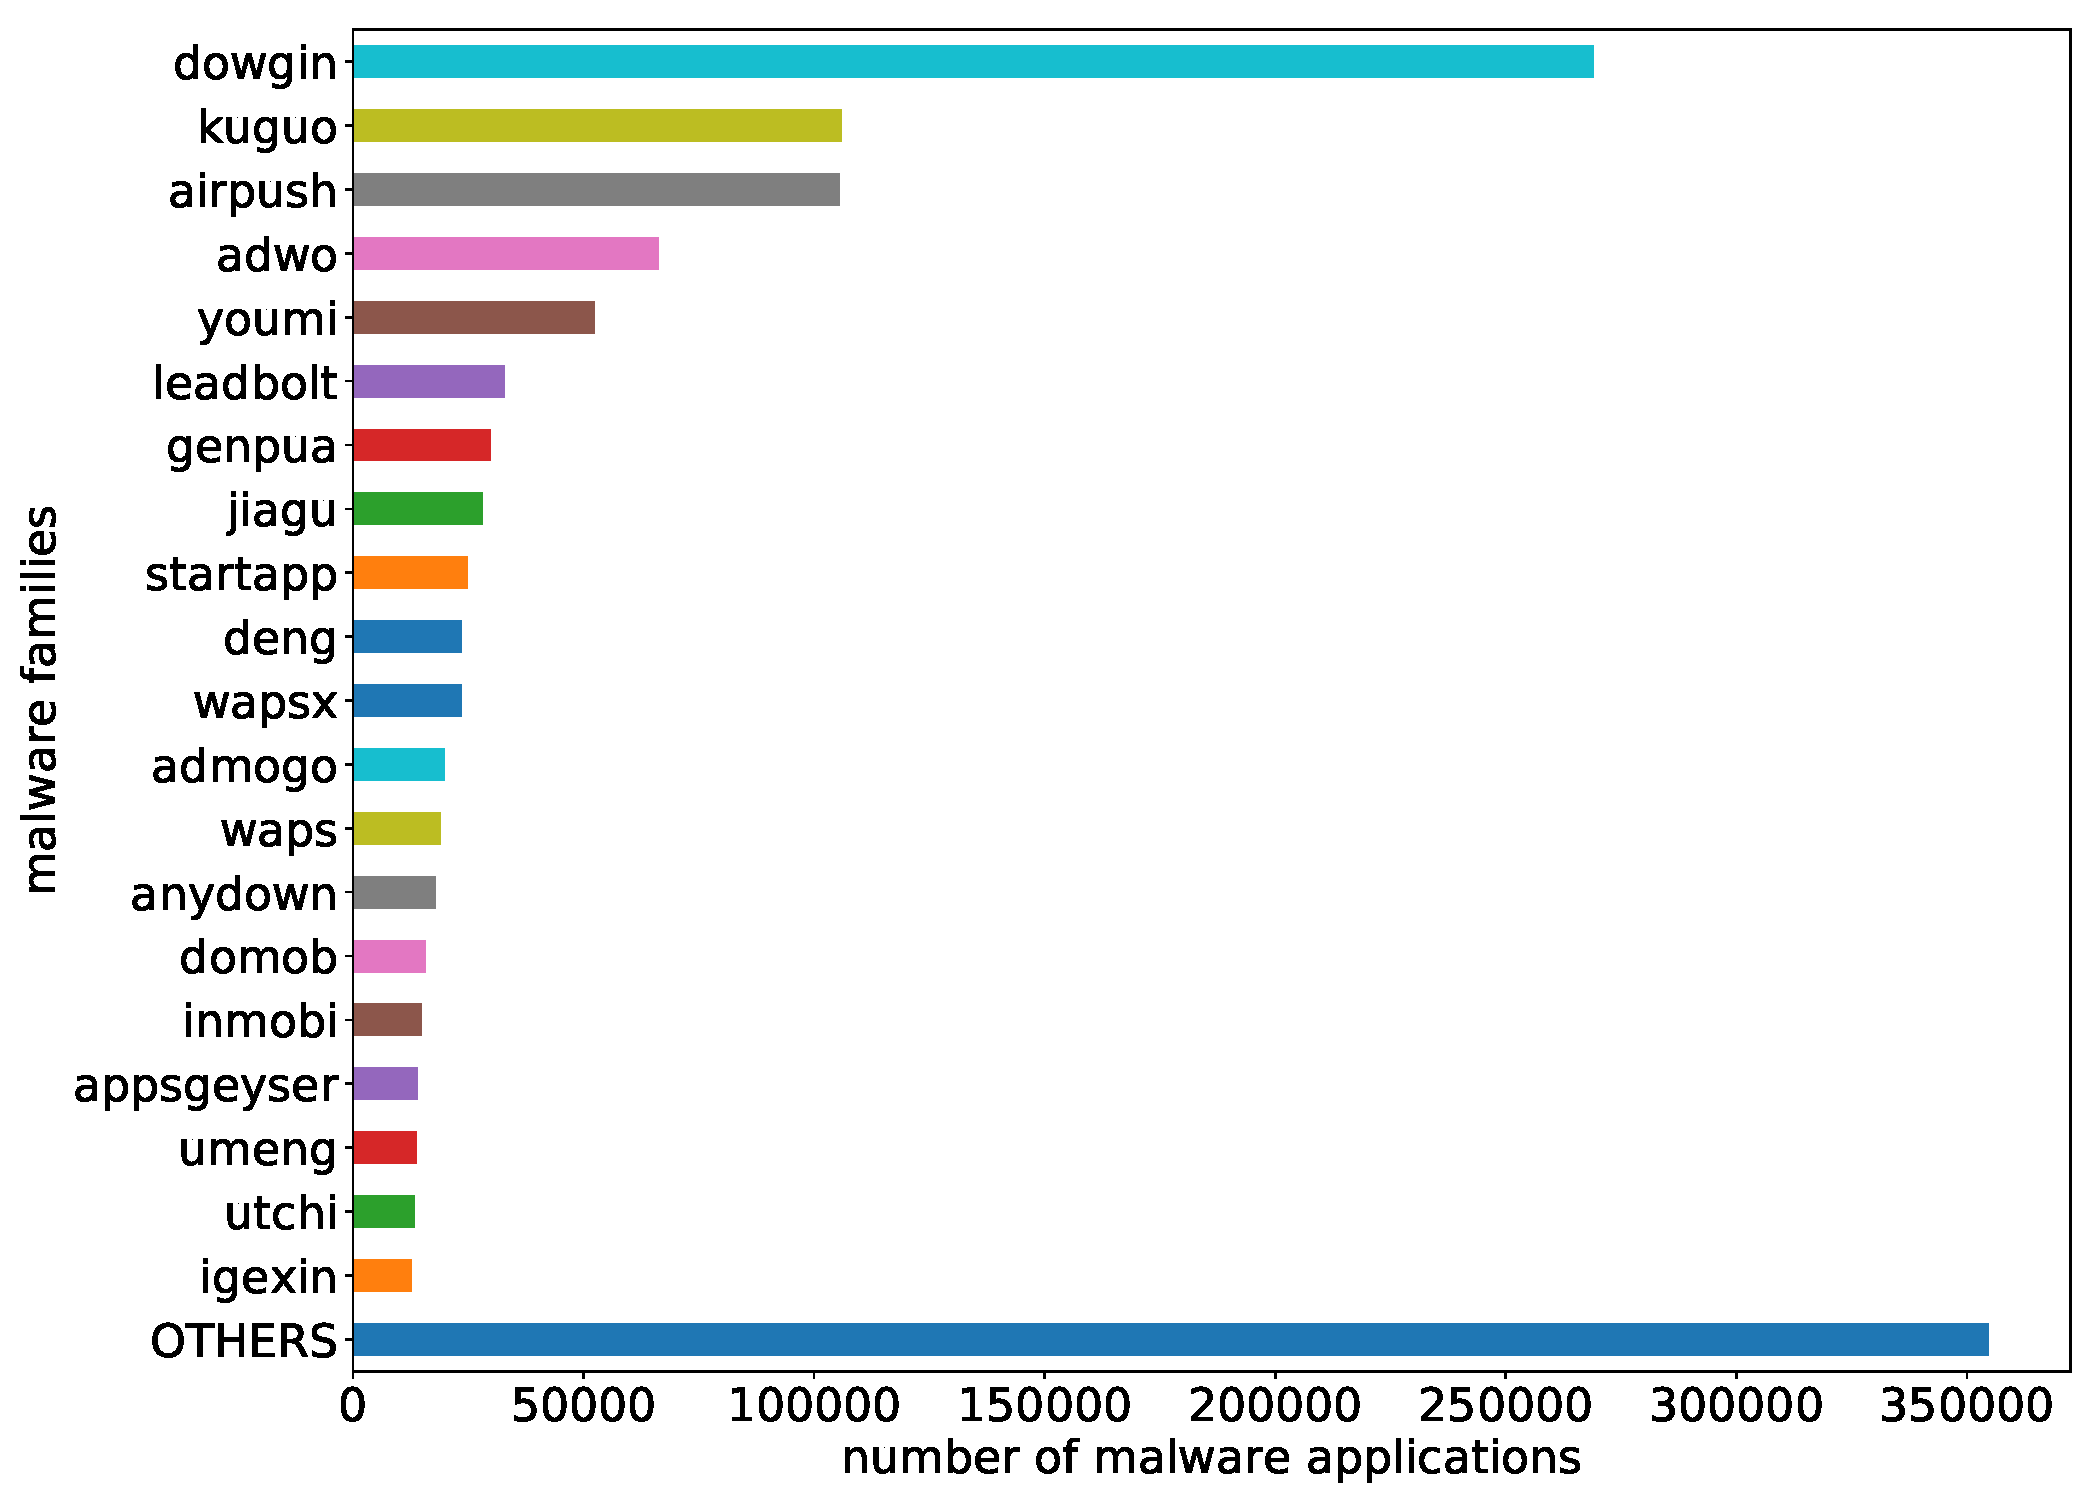
\includegraphics[width=0.85\linewidth]{figures/apgraph/euphony.pdf}
        \caption[Distribution of malware families with at least 100 samples]{Distribution of malware families with at least 100 samples according to Euphony}
	\label{figure:apgraph:families}
\end{figure}

Figure~\ref{figure:apgraph:families} shows the distribution of malware families for the labels unified by Euphony.
We can see that the distribution has a long tail of small families, as \textit{dowgin} dominates the ranking while smaller families are grouped into the OTHERS bin.
In total, Euphony proposes 3600 different malware families for the Androzoo dataset.
Our study focused on the larger 20 families proposed by the following antivirus: ESET-Nod32, Sophos, GData, F-Secure (in addition to Euphony unified names).
Antiviruses are selected in order to maximize the number of positive detections based on Androzoo++ data.
\subsubsection{Artifacts}
The artifacts included in our analysis are extracted with Androguard~\cite{desnos_androguard_nodate}, an open source tool that decompiles Android applications to retrieve their resources and bytecodes.
This tool is classified as a static analysis system, as it does not execute the application on a virtual machine to collect runtime information.
Instead, one of the main benefits of this approach is the global coverage that the solution provides.
Every static component in the application (e.g., strings, methods, files) can be indexed as an artifact identifier by AP-GRAPH.
In total, our evaluation includes 732 million distinct artifacts collected from 1 million malicious applications.
This type of static analysis is also fast and scalable, as it requires only 8 seconds on average for a single machine core to decompile the applications and collect its artifacts.

\begin{figure}[!ht]
        \centering
	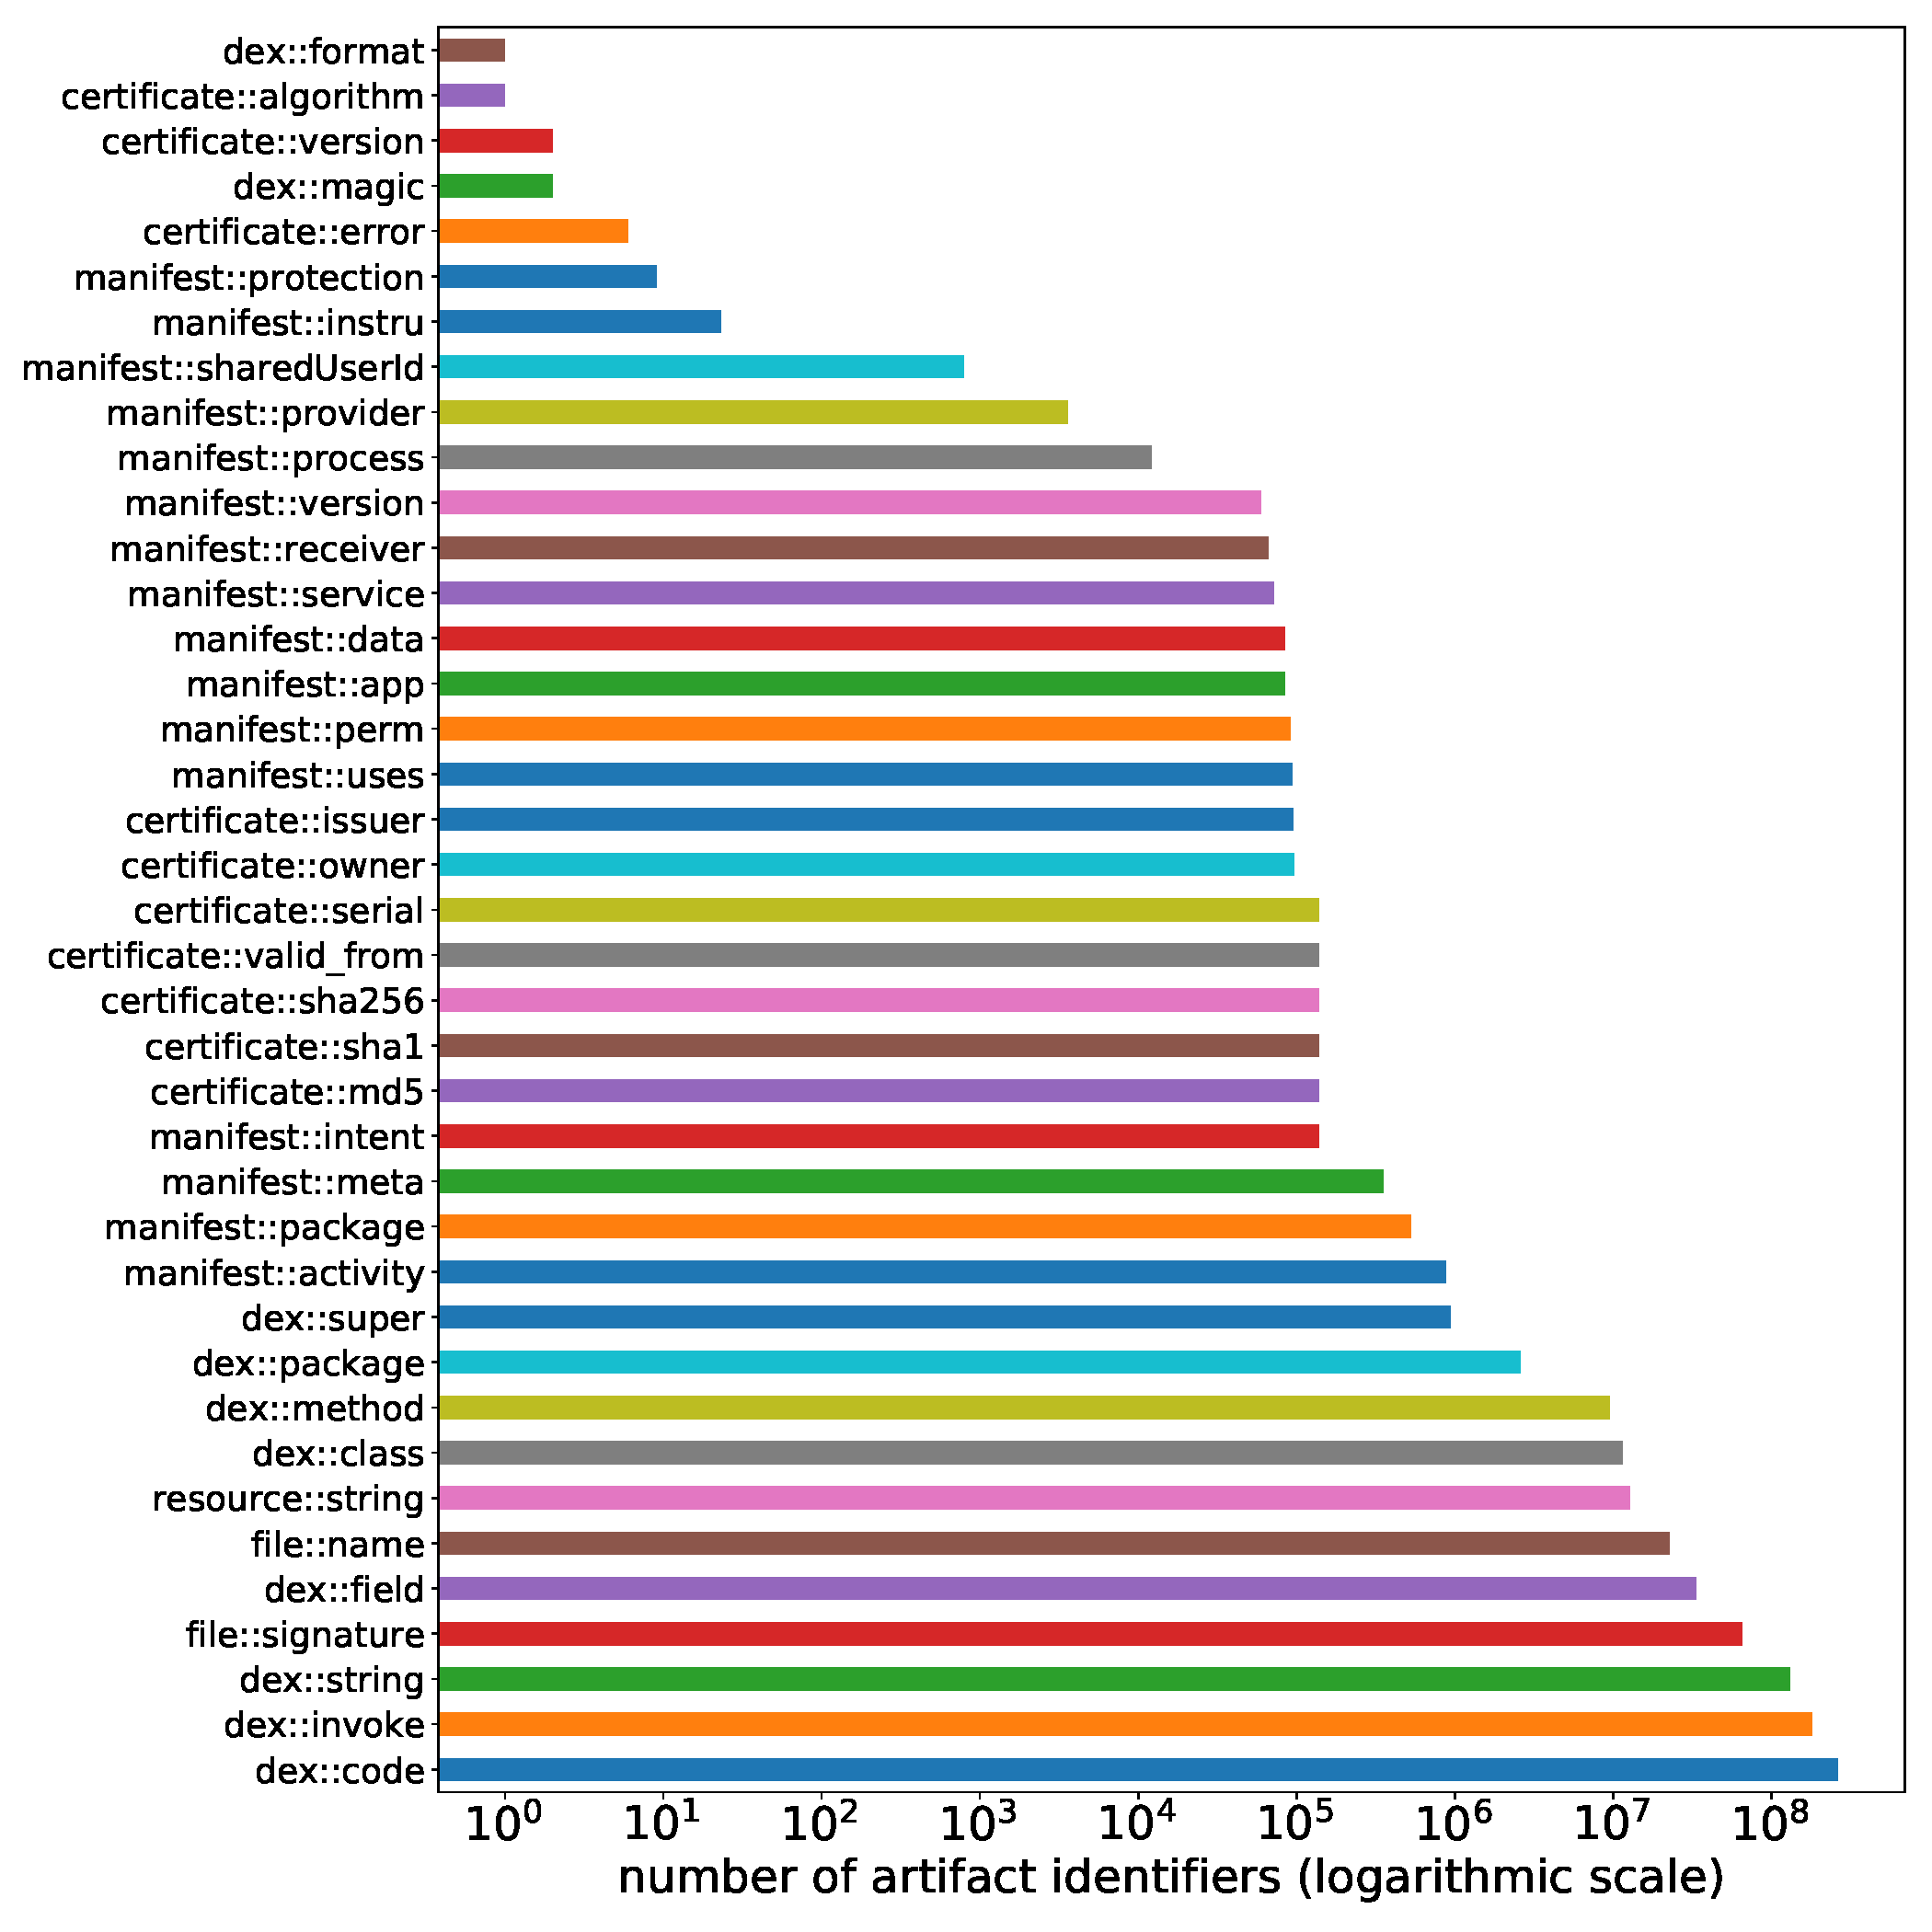
\includegraphics[width=\linewidth]{figures/apgraph/families.pdf}
	\caption{Distribution of artifact identifiers by category}
	\label{figure:apgraph:artifacts}
\end{figure}

The artifacts considered in our analysis are grouped into 46 categories, and displayed in Figure~\ref{figure:apgraph:artifacts}.
Each category is associated with a specific artifact type.
For instance, the strings present in dex files (a packaged version of the application source code) are identified by the entry dex::string.
As another example, the source code of methods is hashed and identified by the entry dex::code.
The listing below provides an overview of the artifact categories covered in our evaluation:

\paragraph{DEX information (starting with dex)}: hash value computed from source codes (\textit{code}), string values (\textit{string}), method invocations (\textit{invoke}), field names (\textit{field}), method names (\textit{method}), class names (\textit{class}), package names (\textit{package}), superclass names (\textit{super}), dex magic number (\textit{magic}), dex format (\textit{format}).

\paragraph{File information (starting with file)}: hash value computed from file content (\textit{signature}), file names (\textit{name}).

\paragraph{Manifest information (starting with manifest)}: activity names (\textit{activity}), service names (\textit{service}), provider names (\textit{provider}), receiver names (\textit{receiver}), process names (\textit{process}), intent names (\textit{intent}), data keys (\textit{data}), metadata keys (\textit{meta}), application package (\textit{package}), application version (\textit{version}), application features (\textit{app}), application libraries and permissions (\textit{uses}), custom permissions (\textit{perm}), user identifier (\textit{sharedUserId}), protection levels (\textit{protection}), instrumentation classes (\textit{instru}).

\paragraph{Resources information (starting with resource)}: string values for both keys and entries (\textit{string}).

\paragraph{Certificate information (starting with certificate)}: SHA1, MD5 and SHA256 signatures (\textit{sha1, md5, sha256 respectively}), beginning of validity period (\textit{valid\_from}), serial number (\textit{serial}), version number (\textit{version}), certificate owner (\textit{owner}), certificate issuer (\textit{issuer}), signature algorithm name (\textit{signature\_algorithm\_name}), certificate errors (\textit{keytool\_error}).
\subsection{Performances}
\subsubsection{Characterization}
To evaluate the capacity of AP-GRAPH in characterizing Android malware, we consider each antivirus and family introduced in the previous section.
For each pair of antivirus and family, we report the artifact which is the most specific of this pair.
For instance, if 5 artifacts $\mathit{a}_1, \mathit{a}_2 ,\mathit{a}_3 ,\mathit{a}_4 ,\mathit{a}_5$ are discriminative of the family $\mathit{t}$ with an occurrence of 100, 200, 300, 400, 500 respectively, $\mathit{a}_5$ is the most specific artifact as it appears in more applications for this family (500 times) than the other artifacts.
We then normalize the number of occurrences by dividing this value with the total number of applications associated with the pair of antivirus and family.

\begin{figure}[!ht]
        \centering
	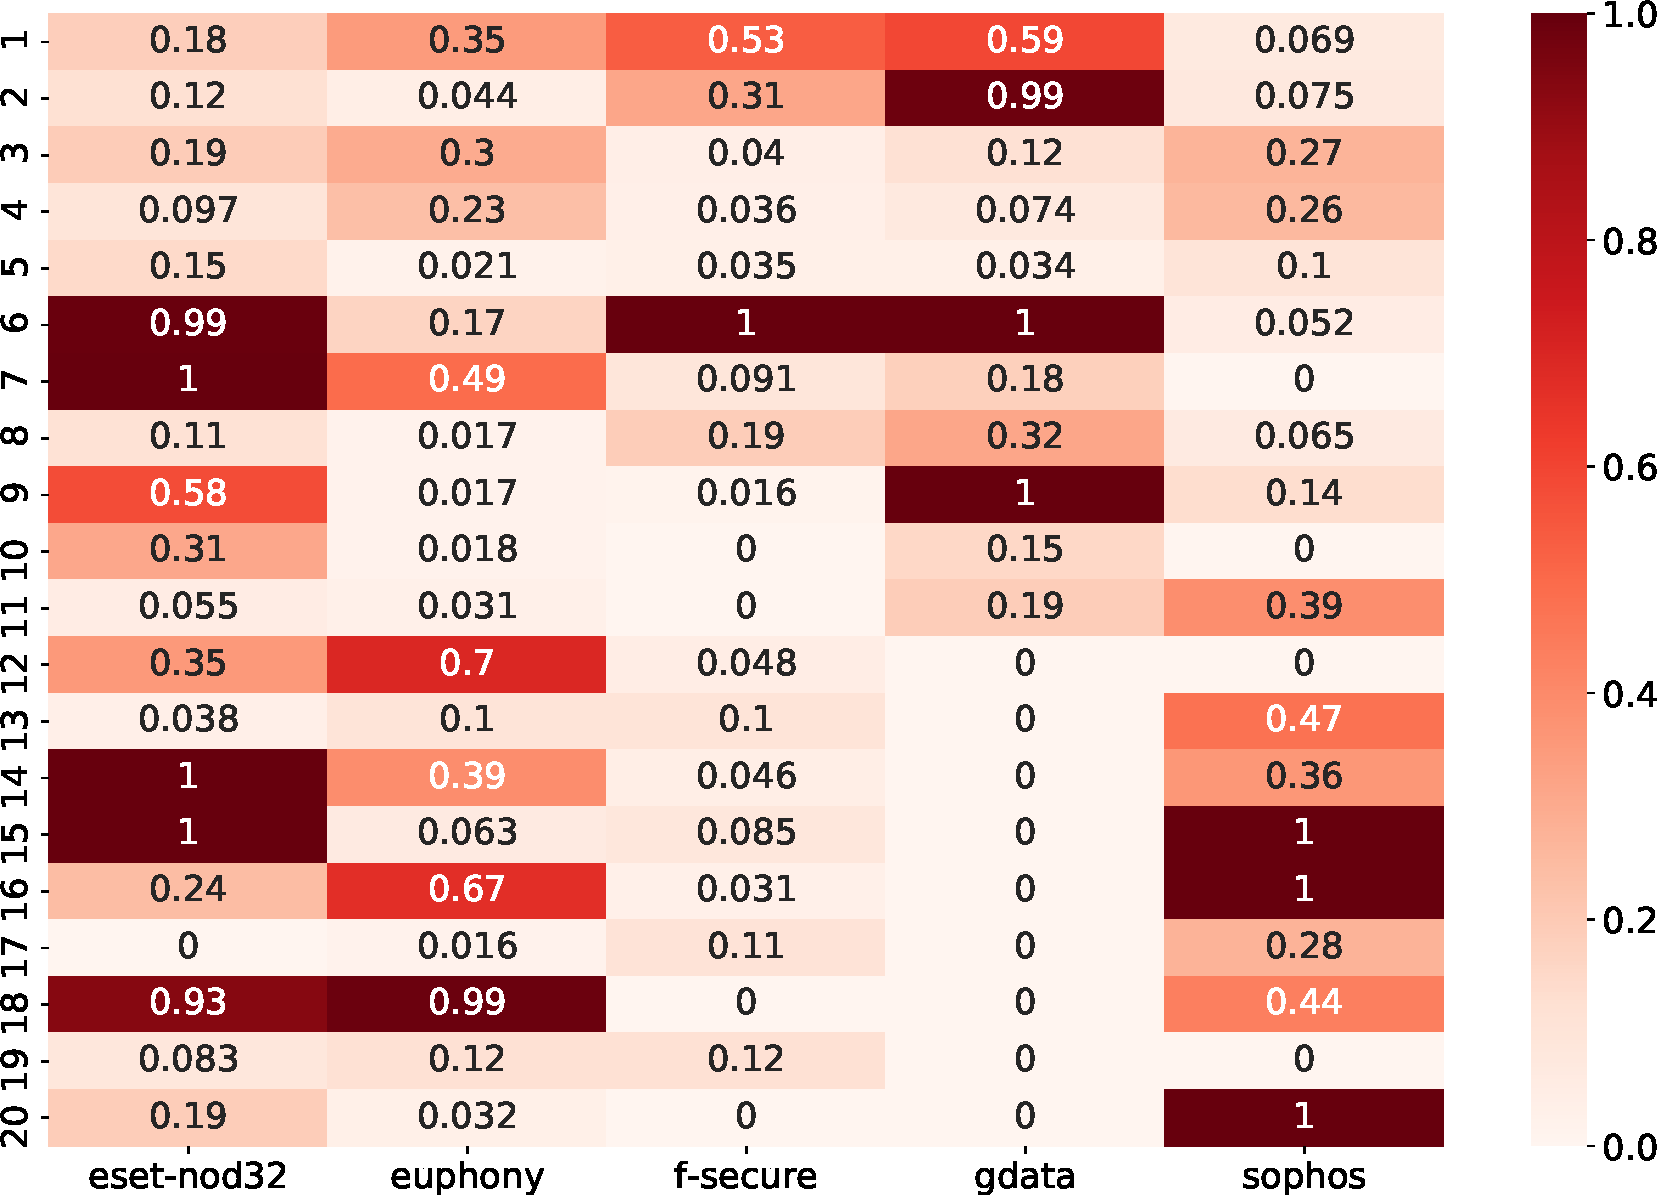
\includegraphics[width=0.85\linewidth]{figures/apgraph/selected.pdf}
        \caption[Maximum proportion of malware identified by AP-GRAPH]{Maximum proportion of malware identified by AP-GRAPH per antivirus (columns) and families (rows)}
	\label{figure:apgraph:char}
\end{figure}

\begin{figure}[!ht]
        \centering
	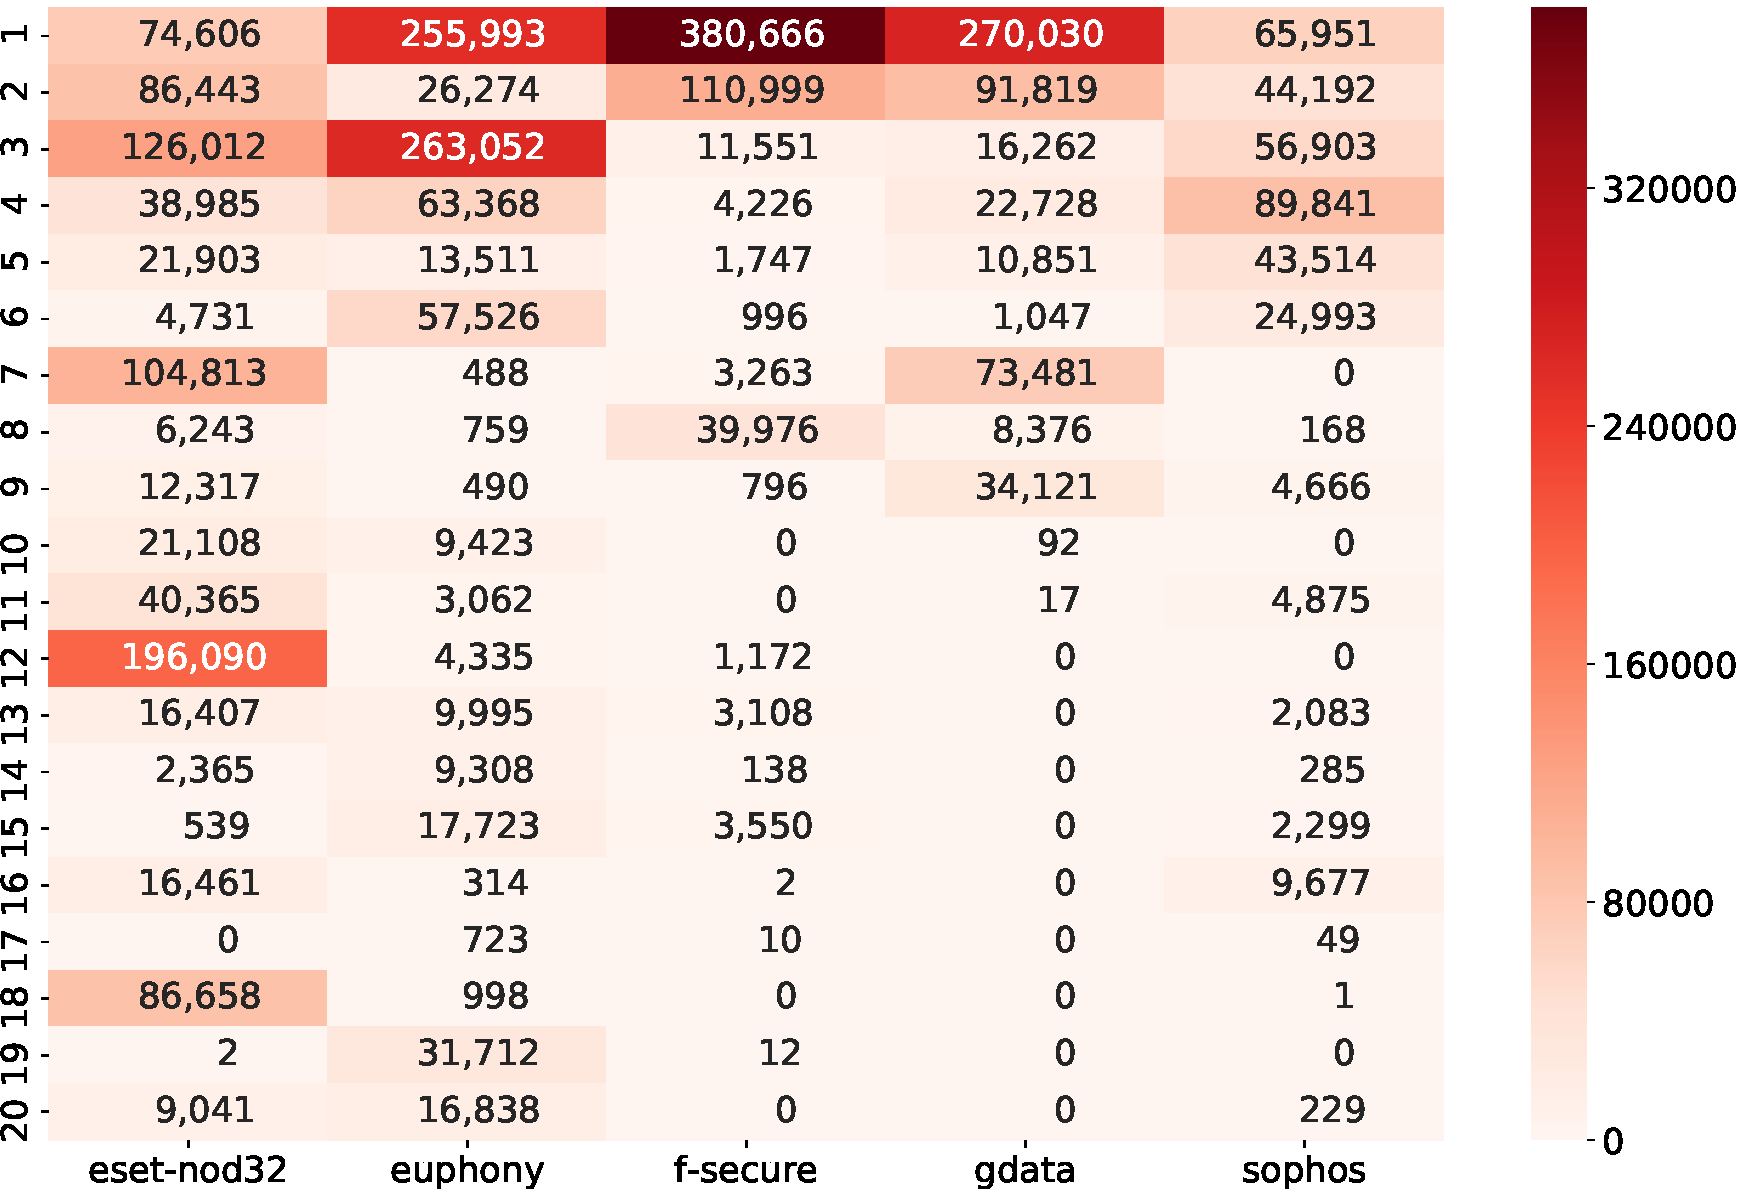
\includegraphics[width=0.85\linewidth]{figures/apgraph/uncovered.pdf}
        \caption[Number of characteristic artifacts discovered by AP-GRAPH]{Number of characteristic artifacts discovered by AP-GRAPH per antivirus (columns) and families (rows)}
	\label{figure:apgraph:count}
\end{figure}

We can see the results of our characterization analysis in Figure~\ref{figure:apgraph:char}.
The values range from 0 (no artifacts were found for the antivirus and family) to 1 (one artifact is present in all samples for this antivirus and family).
For each antivirus (columns), the families (rows) are ordered from the larger (top) to the smaller family (bottom).
As this order is different for each antivirus, we replaced the family names by an ordinal value from 1 to 20.

We observe that AP-GRAPH was able to find some key artifacts that are discriminative of whole families.
This is the case for $\mathit{t}_6, \mathit{t}_7, \mathit{t}_{14}, \mathit{t}_{15}, \mathit{t}_{18}$ of \textit{eset-nod32}, $\mathit{t}_{18}$ of \textit{euphony}, $\mathit{t}_6$ of \textit{f-secure},$\mathit{t}_2, \mathit{t}_6, \mathit{t}_9$ of \textit{gdata}, $\mathit{t}_{15}, \mathit{t}_{16}, \mathit{t}_{20}$ of \textit{sophos}.
These results show that AP-GRAPH can find at least an artifact present in and only in every malicious application of these combinations of antivirus and family.
To complement this analysis, we also display on Figure~\ref{figure:apgraph:count} the total number of characteristic artifacts identified by AP-GRAPH.
This figure shows that out of 100 antivirus and family combinations, 74 combinations have more than 100 characteristic artifacts, 61 combinations have more than 1,000 characteristic artifacts and 39 have more than 10,000 characteristic artifacts.

We also observed from Figure~\ref{figure:apgraph:char} and Figure~\ref{figure:apgraph:count} that some antivirus and families are not fully characterized by the artifacts uncovered by AP-GRAPH.
Multiple reasons could explain this result.
First, antivirus labels may be associated with some hidden artifacts that are not included in this study (e.g., runtime values).
Second, the antivirus labels could contain too much noise or provide information that are not granular enough to find common denominators between them.
Finally, some malware families could be very generic and include a broad set of artifacts present in multiple families.
We discuss the opportunity of improving our characterization scheme in the Discussion section.
\subsubsection{Feature processing}

\begin{figure}[!ht]
        \centering
	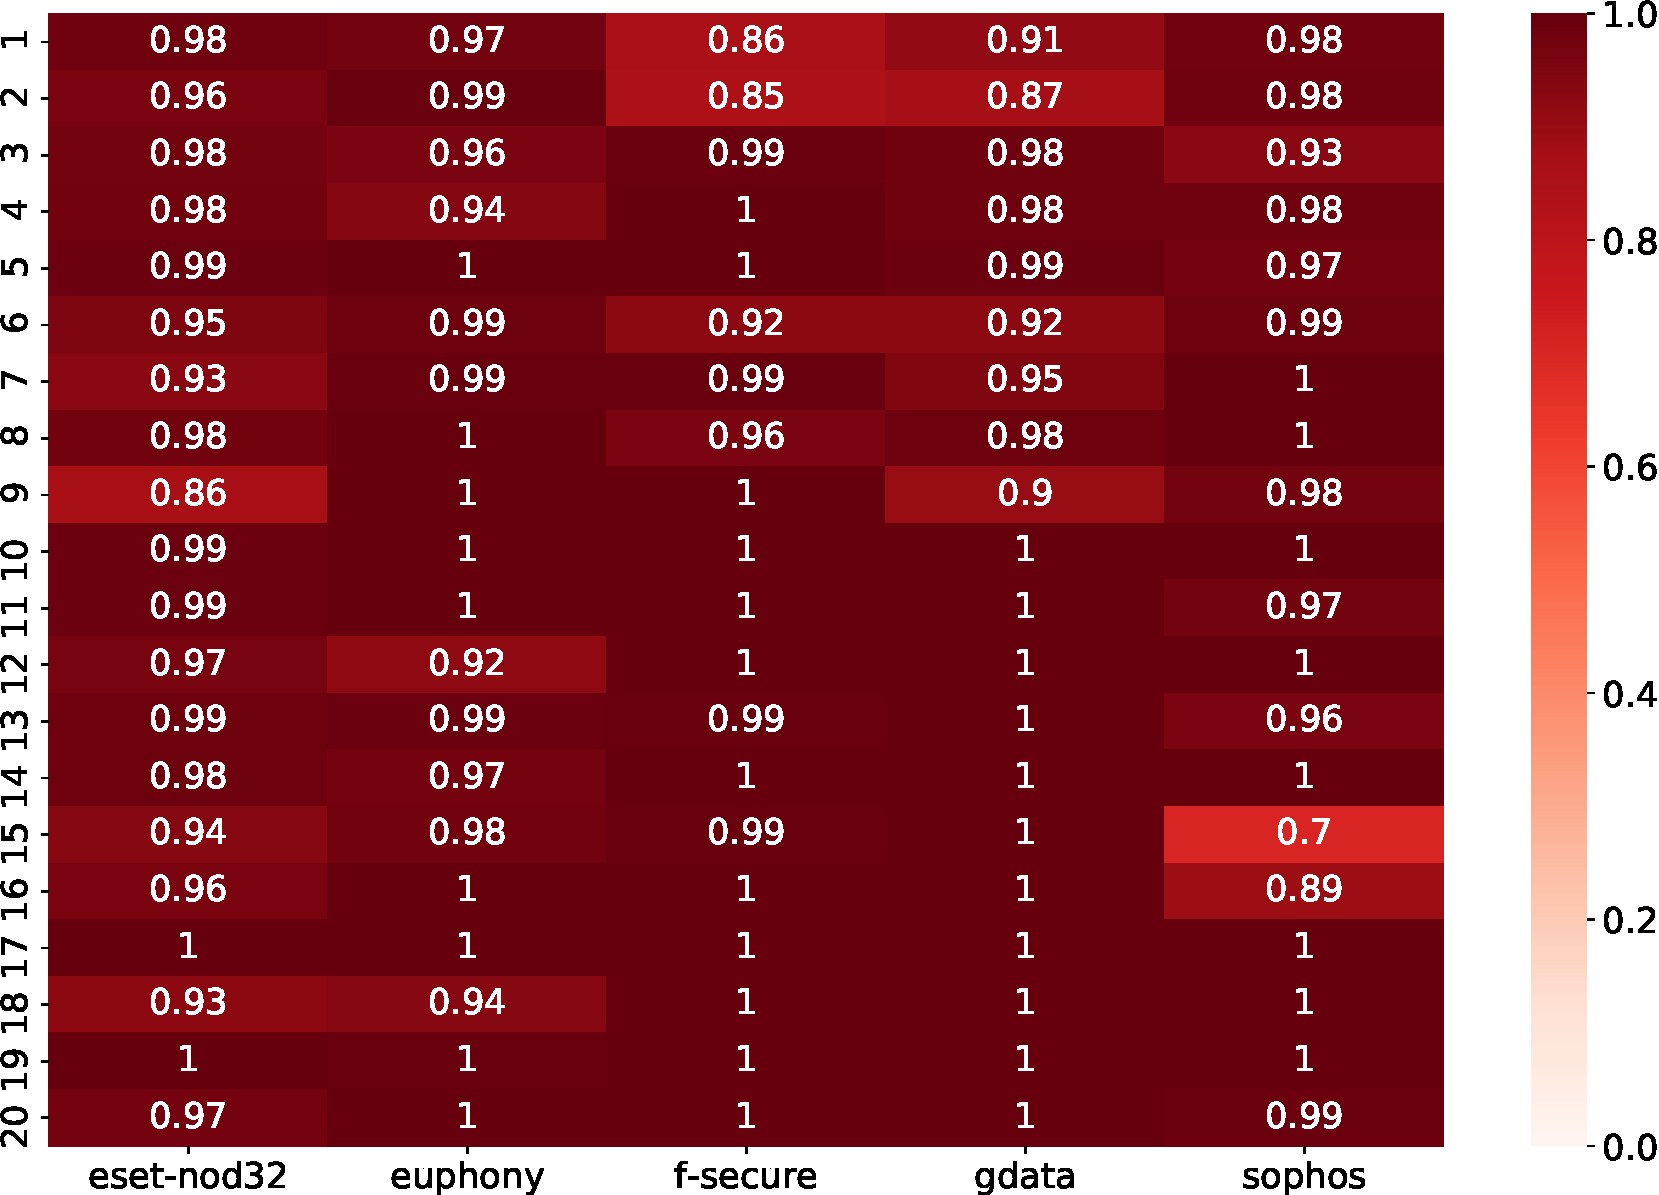
\includegraphics[width=0.85\linewidth]{figures/apgraph/notselected.pdf}
        \caption[Proportion of artifacts dropped by AP-GRAPH]{Proportion of artifacts dropped by AP-GRAPH for each antivirus (columns) and families (rows)}
	\label{figure:apgraph:notsel}
\end{figure}

Selecting relevant features is one of the most challenging aspects of building detection systems based on machine learning.
In this regard, AP-GRAPH can assist practitioners by eliminating artifacts that do not relate to the malware families that these systems must classify.
To evaluate the capacity of AP-GRAPH in filtering these features, we compute for each antivirus and malware families the proportion of artifacts that were dropped by our system as they were found not to be discriminative of any malware family.

We can see in Figure~\ref{figure:apgraph:notsel} the result of our feature processing.
For each cell, a value close to 1.0 means that the number of dropped artifacts is closer to the total number of artifacts associated with the antivirus and family combinations.
We notice that the minimum value on this figure is 0.7 for the 15th most important family of the Sophos antivirus.
Thus, AP-GRAPH can remove a vast majority of artifacts that are not specific to a particular family.
This ability further complements the capacity of AP-GRAPH in characterizing malware families by revealing the artifacts which are NOT associated with a particular behavior.
\subsection{Case studies}
In this section, we consider the particular case of the family \textit{adwo} and the antivirus \textit{gdata}.
This family contains 44,828 applications and corresponds to the result of the second row and fourth column in Figure~\ref{figure:apgraph:char}.
The next parts will present the artifacts selected by AP-GRAPH for this family and the reverse analysis of a single application taken at random from Androzoo dataset.
\subsubsection{Distinctive artifacts}

\begin{table}[t]
	\centering
        \caption[Most specific artifacts identified by AP-GRAPH]{Most specific artifacts identified by AP-GRAPH for the family \textit{adwo} of antivirus \textit{gdata}}
	\resizebox{\linewidth}{!}{
		\begin{tabular}{|c|c|c|c|}
			\hline
                        \textbf{Location} & \textbf{Type}     & \textbf{Name}                                                      & \textbf{found}  \\
			\hline
			manifest & activity & adwoadbrowseractivity                                     & 44,162 \\
			dex      & invoke   & com/adwo/adsdk/i-><init>                                  & 33,889 \\
			dex      & invoke   & com/adwo/adsdk/h-><init>                                  & 33,078 \\
			dex      & class    & FSAd                                                      & 32,551 \\
			dex      & invoke   & com/adwo/adsdk/AdwoSplashAdActivity->requestWindowFeature & 32,541 \\
			dex      & invoke   & com/adwo/adsdk/AdwoSplashAdActivity->getWindow            & 32,541 \\
			dex      & string   & lcom/adwo/adsdk/fsad;                                     & 32,536 \\
			dex      & code     & \#583b5                                                   & 32,536 \\
			% 583b5fd78b12ede179b48081829a1a9af8a94d3fc67a9a6ff7867f24e77524db
			dex      & invoke   & com/adwo/adsdk/FSAd-><init>                               & 32,536 \\
			dex      & string   & http://r2.adwo.com/adfs                                   & 32,518 \\
			dex      & string   & vlijlzzz                                                  & 32,505 \\
			dex      & code     & \#1b25f                                                   & 32,485 \\
			% 1b25f41d647d7eb684fbb0933860626e7ce75c34120aca1a34b0e20e08f09c94
			dex      & invoke   & com/adwo/adsdk/V-><init>                                  & 32,268 \\
			dex      & code     & \#de7d0                                                   & 32,103 \\
			% de7d02b09733bd70de518444c54464cf6d41c3a9effa23664a47c68ac2f8a1c4
			dex      & code     & \#baf7b                                                   & 32,103 \\ %%%%%%%%%%%%%
			% baf7be622bb53166edace516ffa985ed2e687bc6ab29536869d1eb709573c9a6
			dex      & string   & malformed click url.will try to follow anyway.            & 32,093 \\
			dex      & invoke   & com/adwo/adsdk/AdwoAdBrowserActivity->a                   & 32,090 \\
			dex      & string   & fsad.htmlcontent                                          & 32,090 \\
			dex      & code     & \#e5b18                                                   & 32,088 \\
			% e5b1813a1be7d3a04b2dfb2c4a6da8dabec3b0e287ec421a4d30f3efd1413811
			dex      & invoke   & com/adwo/adsdk/AdwoSplashAdActivity->a                    & 32,023 \\
			\hline
		\end{tabular}
	}
	\label{table:apgraph:rev}
\end{table}


The artifacts identified by AP-GRAPH are listed on Table~\ref{table:apgraph:rev}.
Each row contains the location, type, name, and the number of times this artifact was found in the family.
As an example, the first row shows that the activity AdwoAdBrowserActivity located in the Manifest file was found in 44,162 applications out of the 44,828 applications of the family (98\%).
The fourth row corresponds to the class FSAd present in the DEX file and included in 32,551 applications of the family (72\%).

We see from this table that most entries are related to the family, as the artifacts contain its name.
This is the case for the invoke calls that start with com/adwo and the activity AdwoAdBrowser.
We can also notice a URL encoded as a string that contains the domain name r2.adwo.com.
These artifacts are good indicators that AP-GRAPH can retrieve components which are related to the family under investigation.
However, while some artifacts can be explained from their identifiers, others are more obscure and require some manual analysis.
We explore these elements uncovered by AP-GRAPH in the next part of this section.
\subsubsection{Reverse engineering}
To demonstrate the assistance that AP-GRAPH provides in reversing malicious applications, we selected a single application at random from our set and analyzed the content of its artifacts.
As a starting point, we considered every application associated with the list of artifacts showed in Table~\ref{table:apgraph:rev}, which corresponds to the antivirus gdata and the family adwo.
The SHA256 signature of the application is \seqsplit{000A0B1022EC485473DFAACA433F9548911BC7089B6A3C7B47F9EC5541005CA1}.

\begin{figure}[!ht]
        \centering
	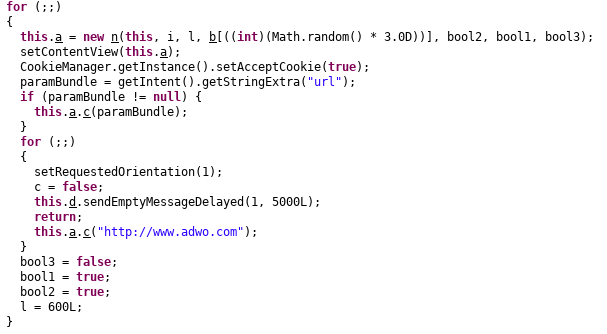
\includegraphics[width=\linewidth]{figures/apgraph/contact.png}
	\caption{The application contacts the primary server to download the ads}
	\label{figure:apgraph:contact}
\end{figure}

In Figure~\ref{figure:apgraph:contact}, we analyzed the content of the \textit{onCreate} method of the AdwoAdBrowserActivity, as is it the first artifact reported by AP-GRAPH.
We notice that this method constructs an object of class n and contacts the adware server at the URL: http://www.adwo.com.

\begin{figure}[!ht]
        \centering
	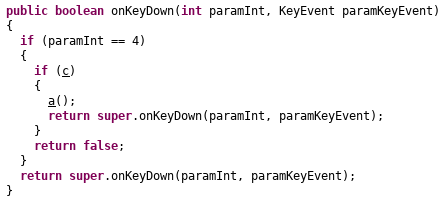
\includegraphics[width=0.75\linewidth]{figures/apgraph/listener.png}
	\caption{The application setups the event listener to trigger the ads}
	\label{figure:apgraph:listener}
\end{figure}

The method that triggers the ads on the screen can be found in class AdwoSplashAdActivity, another artifact identified by AP-GRAPH in Table~\ref{table:apgraph:rev}.
We show the content of this method in Figure~\ref{figure:apgraph:listener}.
It corresponds to the \textit{onKeyDown} method that was identified by AP-GRAPH under the code identifier \seqsplit{BAF7BE622BB53166EDACE516FFA985ED2E687BC6AB29536869D1EB709573C9A6} (or \#baf7b in Table~\ref{table:apgraph:rev}).
We do not know what the variable c controls in this context, but its value is responsible for triggering the advertisement associated with this activity.

\begin{figure}[!ht]
        \centering
	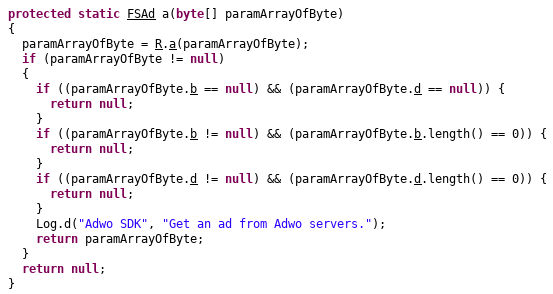
\includegraphics[width=0.9\linewidth]{figures/apgraph/ads.png}
	\caption{The application constructs the ads from an array of bytes}
	\label{figure:apgraph:ads}
\end{figure}

We also analyzed the class FSAd, as it is the fourth artifacts identified by AP-GRAPH in Table~\ref{table:apgraph:rev}.
The content on its constructor, displayed in Figure~\ref{figure:apgraph:ads}.
It shows the construction of the advertisement from an array of bytes (we deduce this behavior from the log entry created inside the constructor).
This method could be monitored to retrieve the content of the ads display to the user.

From our analysis of the application, we see that AP-GRAPH was able to characterize:

\begin{itemize}
	\item the class responsible for contacting the adware server (AdwoAdBrowserActivity)
	\item the method responsible for triggering the ads (\textit{onKeyDown})
	\item the class responsible for handling the content of the add (FSAd)
\end{itemize}

Given these information, an analyst can quickly prioritize the artifacts that are specific to a group of applications and explore their content at a faster pace.
\section{Evolution of malware families over time}
As a first attempt to monitor the deployment of artifacts by malware authors over time, this section presents a short analysis of the evolution of three pairs of antivirus and malware family.
The goal of this section is to illustrate how artifacts proposed by AP-GRAPH can be used to spot anomalies in the development of popular malware families and lead to further investigations.

Each figure contains information about 60 prominent artifacts identified by AP-GRAPH within a given malware family.
We compare their distribution with the total number of Android applications classified for the same malware family in our dataset.
\subsection{ESET NOD32 - Igexin}

\begin{figure}[!ht]
        \centering
	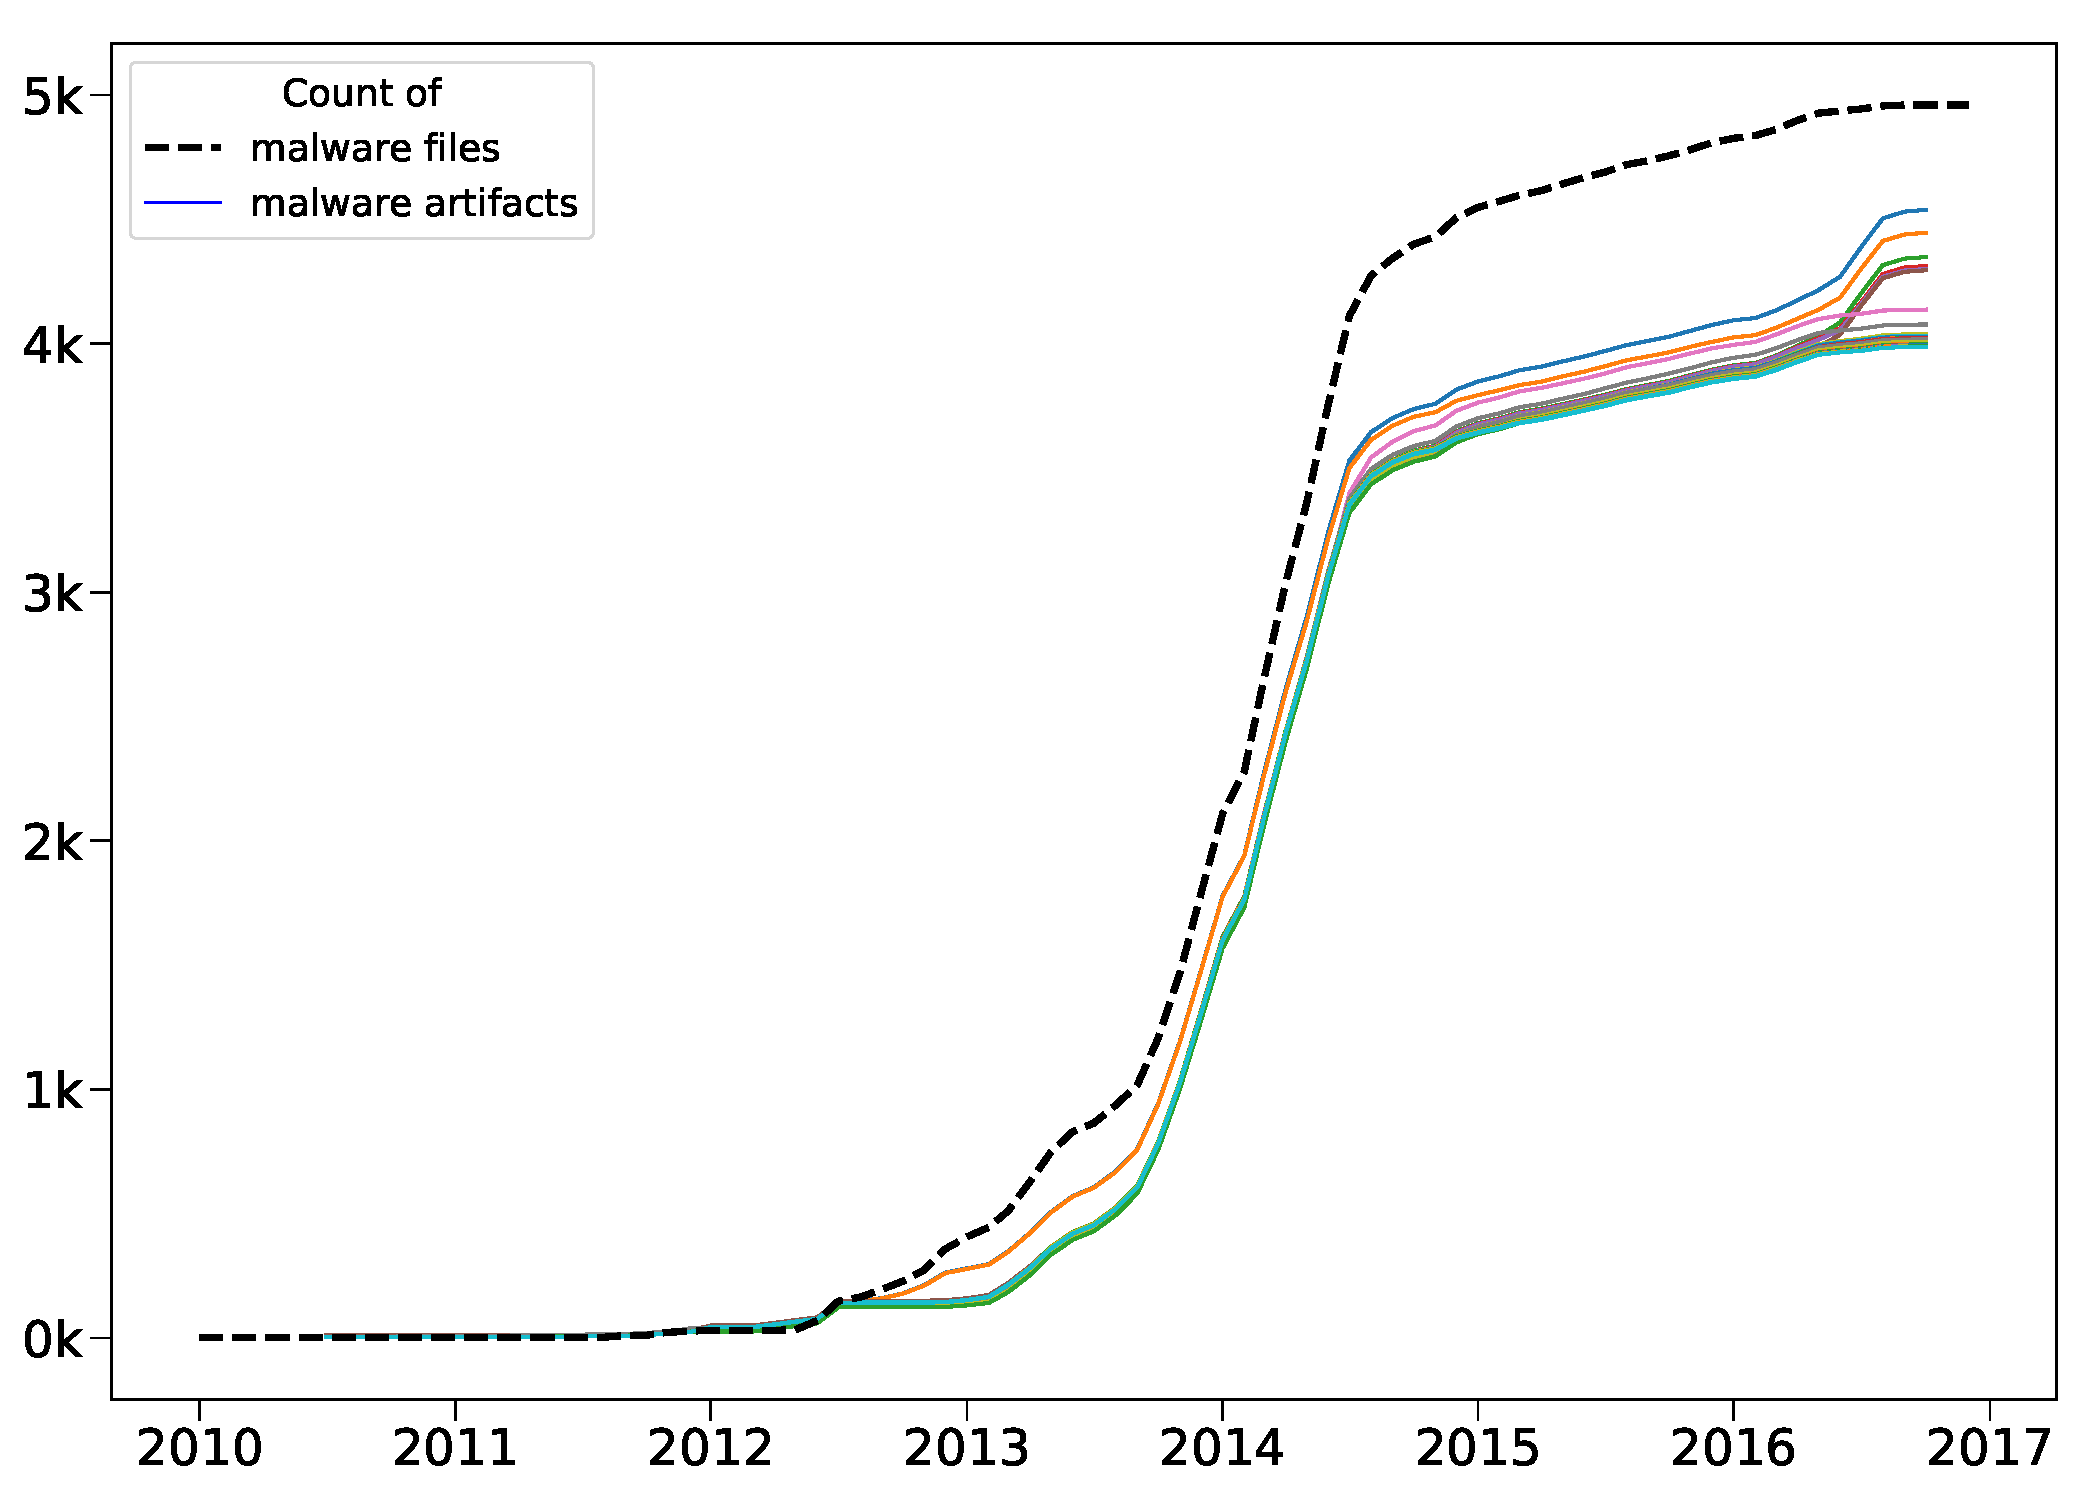
\includegraphics[width=0.85\linewidth]{figures/apgraph/artifacts/eset-nod32_igexin.pdf}
        \caption[Evolution of artifacts identified by AP-GRAPH for ESET NOD32 - Igexin]{Evolution of 60 artifacts identified by AP-GRAPH compared to the total number of malware files associated with the family ESET NOD32 - Igexin}
	\label{figure:apgraph:artifacts:igexin}
\end{figure}

Figure~\ref{figure:apgraph:artifacts:igexin} represents an evolution of malware artifacts that coincides with the release of new malware samples associated with the family.
We can see from 2010 to 2014 that the number of artifacts follows the number of malware files, even when the number of files increases considerably in 2013.
However, a gap starts to appear after 2014 as the number of malware files continues to grow while the number of artifacts associated with the family stagnates.

Malicious applications found in this gap are interesting for a human analyst, as their presence is not tracked by the indicators currently revealed by AP-GRAPH.
This difference could explain a drop of performance in machine learning algorithms or the presence of a new variant derived from the previous version of Igexin.
We can further note that the number of artifacts starts to catch up by the end of 2017 for an unknown reason.
\subsection{EUPHONY - AppsGeyser}

\begin{figure}[!ht]
        \centering
	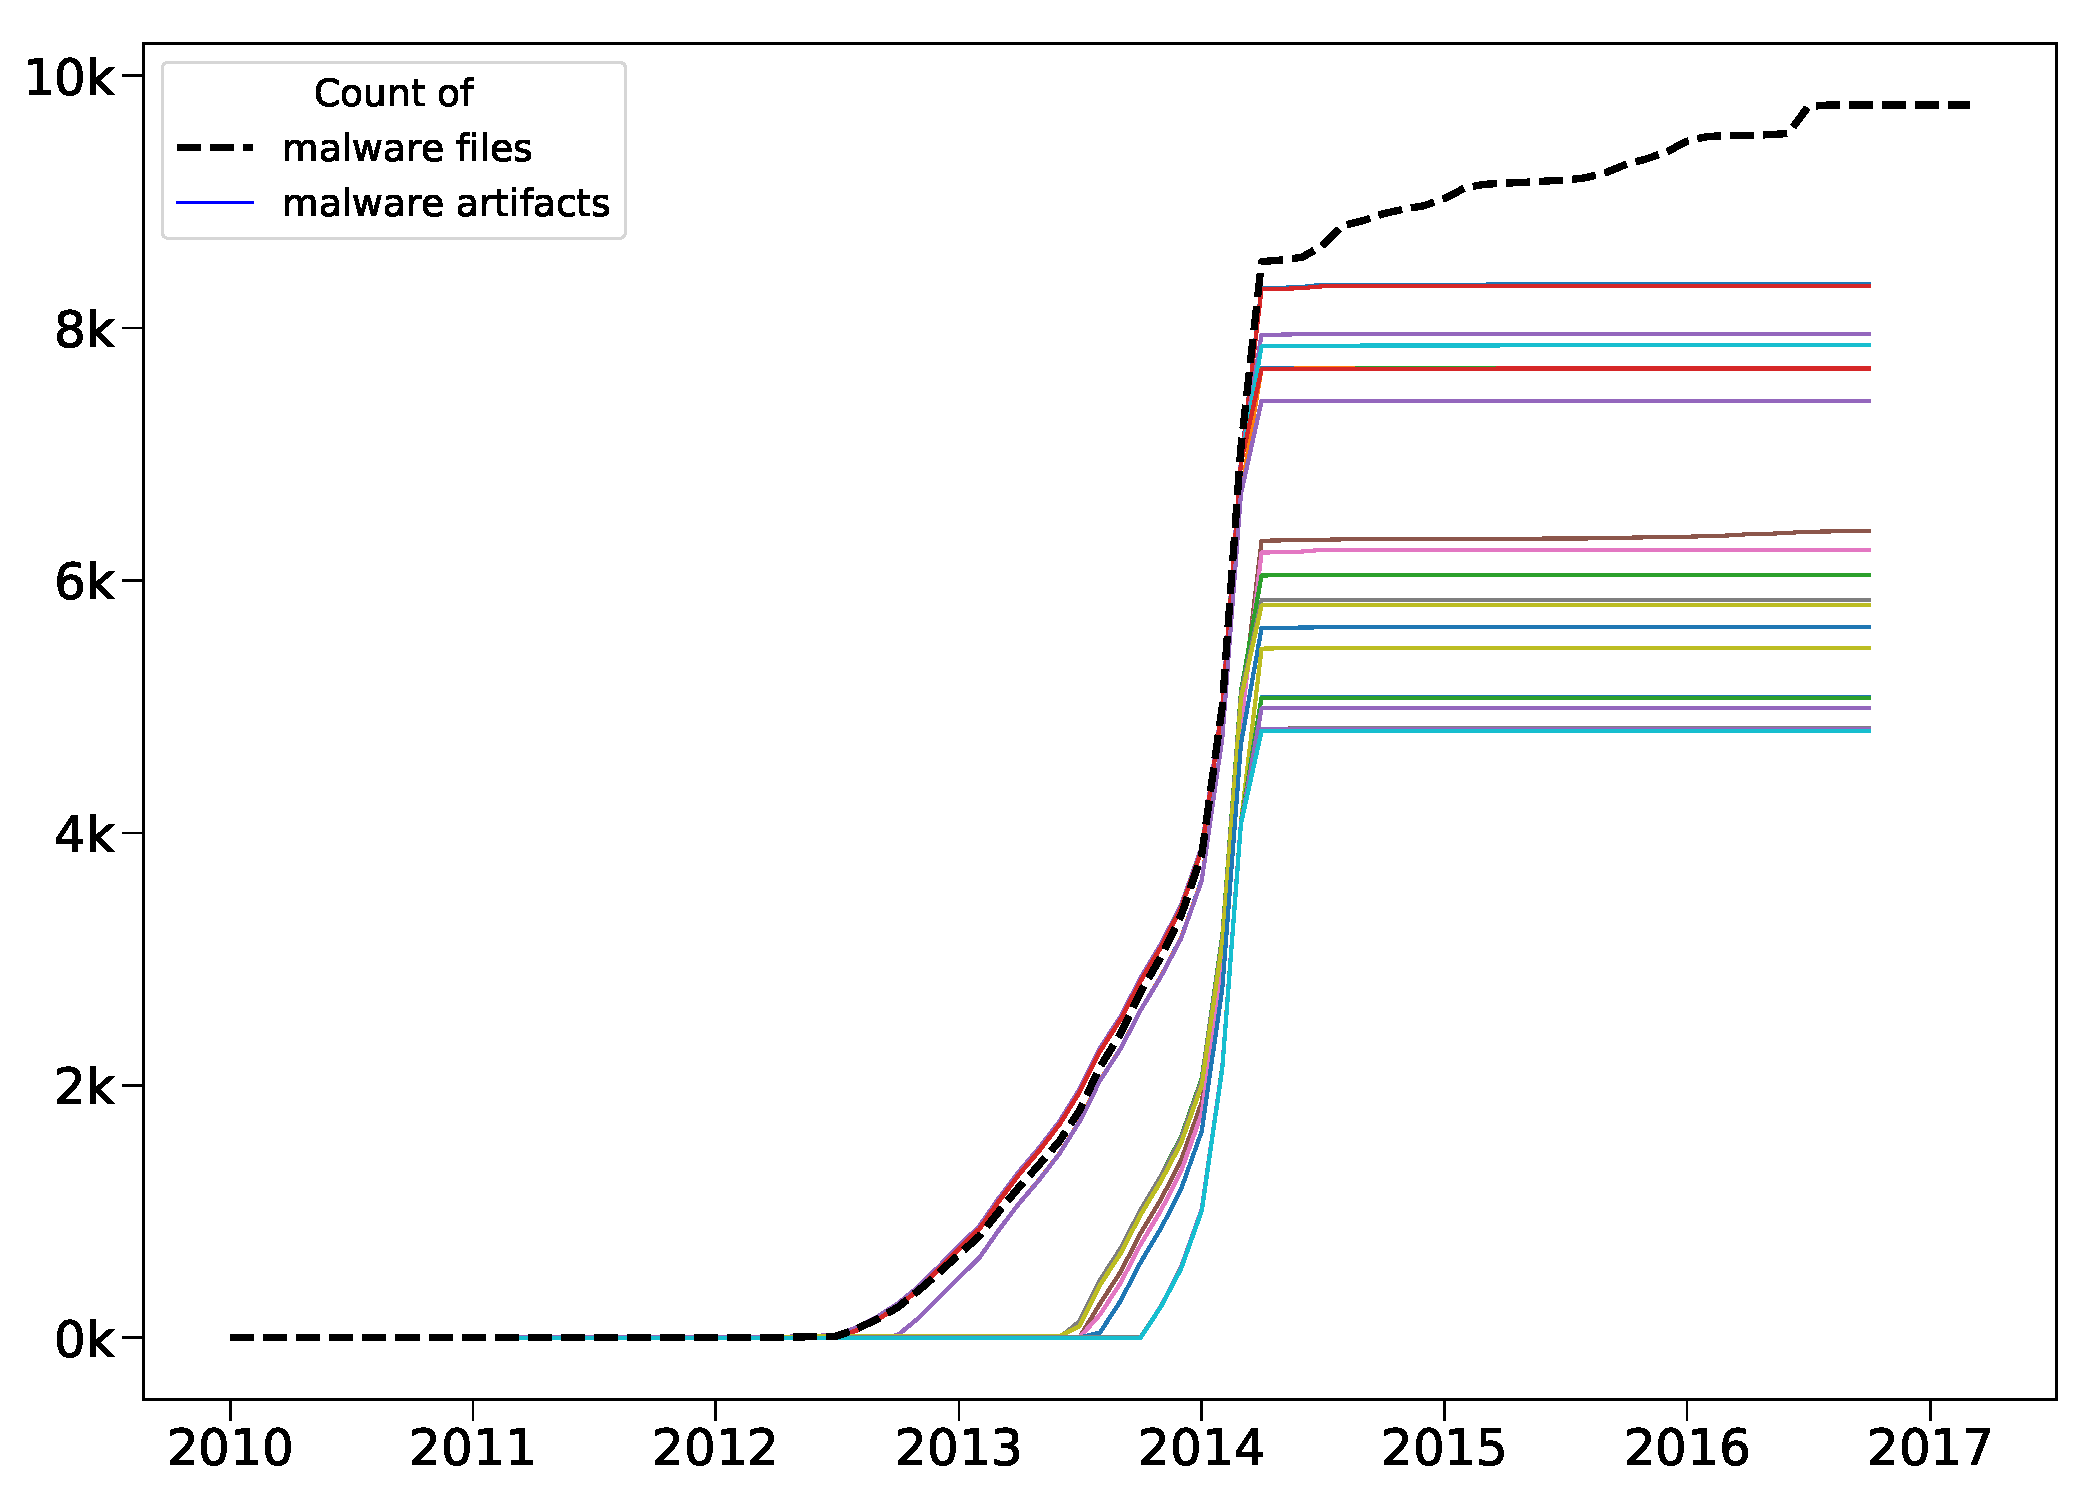
\includegraphics[width=0.85\linewidth]{figures/apgraph/artifacts/euphony_appsgeyser.pdf}
        \caption[Evolution of artifacts identified by AP-GRAPH for EUPHONY - AppsGeyser]{Evolution of 60 artifacts identified by AP-GRAPH compared to the total number of malware files associated with the family EUPHONY - AppsGeyser}
	\label{figure:apgraph:artifacts:appsgeyser}
\end{figure}

Figure~\ref{figure:apgraph:artifacts:igexin} displays a more difficult use cases of malware evolution.
On the one hand, we observe that malware artifacts associated with this family are scattered around the y-axis, indicating a difference in the composition of the malware in this set.
On the other hand, we notice that artifact lines start to become flat in 2014 while the number of malware samples associated with the malware family increases.

This figure reveals either that the malware family used a completely different set of artifacts after 2014 or that artifacts were obfuscated to circumvent defense mechanisms.
Such a scenario could force the investigation of new artifacts to track the malware family during its transformation period.
\subsection{G DATA - SMSpay}

\begin{figure}[!ht]
        \centering
	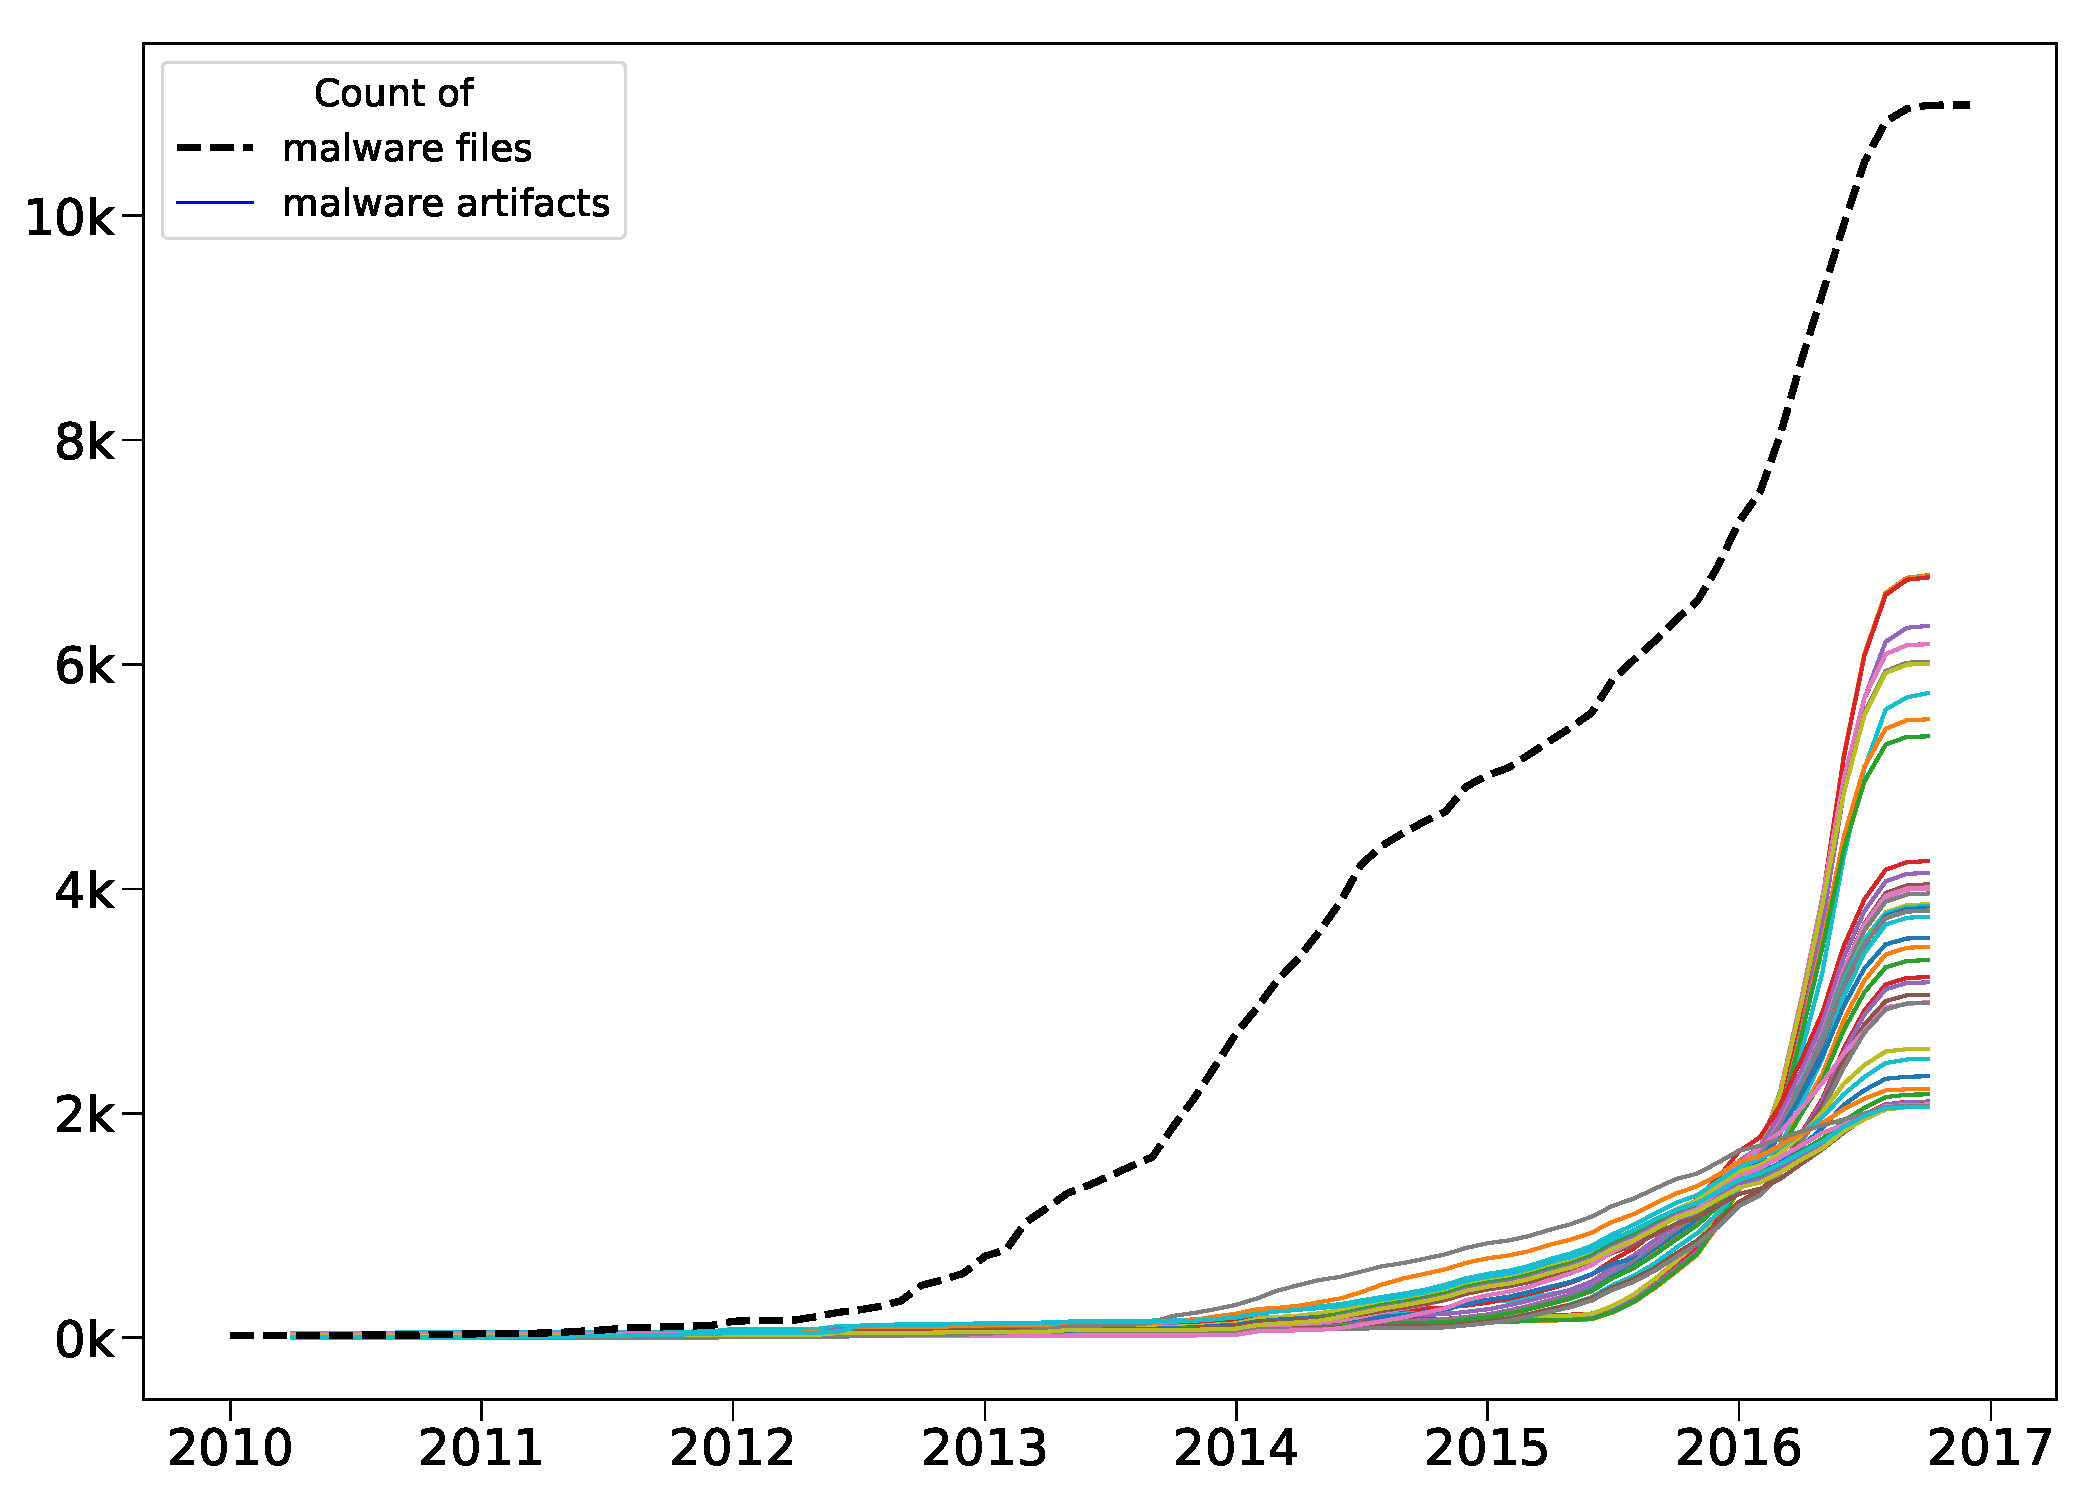
\includegraphics[width=0.85\linewidth]{figures/apgraph/artifacts/gdata_smspay.pdf}
        \caption[Evolution of artifacts identified by AP-GRAPH for G Data - SMSpay]{Evolution of 60 artifacts identified by AP-GRAPH compared to the total number of malware files associated with the family G DATA - SMSpay}
	\label{figure:apgraph:artifacts:smspay}
\end{figure}

Figure~\ref{figure:apgraph:artifacts:smspay} shows a different use case as the artifacts identified by AP-GRAPH were found after 2016, long before the rise of the malware family.
Thus, we observe a period of 3 years during which no specific artifacts could be found to track the evolution of the family accurately.

The most plausible explanation is that AP-GRAPH was able to catch a new variant after 2016, but not beforehand.
Otherwise, it could indicate that malware of this family were more generic before 2016, and that a recent change introduced specific artifacts that could be tracked with AP-GRAPH.
\section{Challenges of malware classification}
\subsection{Obfuscation and variations}
We noted in our study that a high proportion of malware is obfuscated by a simple scheme, including class or method renaming.
Similar to other static analysis approaches, tracking the link between the original and the obfuscated content remains a challenging task.
On the one hand, obfuscation techniques can make the indexing of artifacts more complicated.
On the other hand, these techniques can lead to an explosion of features and introduce a wide variety of unrelated artifacts.
To avoid these constraints in the short term, our study includes a diverse set of artifacts related to the same objects.
For instance, a method is referenced both by its name and the hashing of its code instruction.
Similarly, external files are indexed by their name and also by a sha256 signature based on their content.

Still, the mitigation techniques we adopted in our analysis cannot wholly prevent the impact of obfuscation.
To handle this problem in the long term, new approaches must be designed to find artifacts whose original structure are related.
One of the main benefits of AP-GRAPH in this context is its independence to a predefined type of analysis.
Dynamic or other analysis can be used as an input to AP-GRAPH, as long as these techniques produce identifiers that can be indexed in our database.
Thus, we think AP-GRAPH can be a viable technique to verify that newer analysis techniques can break the obfuscation scheme of malware.
\subsection{Noisy antivirus classifications}
In the evaluation section, we observed that AP-GRAPH could extract discriminative artifacts for some families, while other families do not yield artifacts specific to their whole population.
Multiple reasons could explain these results:

\begin{enumerate}
	\item the artifacts adopted by antivirus vendors are different from the one we used in our evaluation
	\item obfuscation schemes are deployed at large scale by malware authors to bypass the type of analysis we applied in our evaluation
	\item the malware families proposed by antivirus vendors do not reflect the malicious artifacts included in Android malware
\end{enumerate}

For the first and second scenario, finding the right combination of artifacts would be sufficient to solve the detection issue.
Indeed, if antivirus vendors rely mostly on dynamic analysis to detect Android malware, AP-GRAPH could consume these artifacts and verify that they correspond to a known malware family.
The best approach, in this case, would be to test AP-GRAPH with other features and classifiers until a good match is found between the two sets.

The same cannot be said however for the third scenario.
As there is no reference information to assess the results of our evaluation, we cannot guarantee that there is a link to be found between artifacts and the malware families reported by antivirus vendors.
This lack of transparency has an impact on our research community, as we cannot verify that the input we feed to our algorithm is grounded in something concrete.
If this is the case, our community must continue its work on creating better and more transparent malware ground truth.
\subsection{Going from correlation to causation}
Establishing the correlation between malware applications and their artifacts grants us the opportunity to explore what is the cause of their malicious behaviors.
Future works could investigate the artifacts we uncovered to find if they are the root cause or at least trigger some malicious activity.
Our approach also enables the exploration of malware over time to visualize the correlation between malicious applications and their artifacts.
Searching for trends could provide a better picture of the current malware landscape and guide the deployment cycle of more accurate detection models.
